%%%%%%%%%%%%%%%%%%%%%%%%%%%%%%%%%%%%%%%%%%%%%%%%%%%%%%%%%%%%%%%%%%%%%%%%%%%%%%%%%%%%%%%%%%%%%%%%%%%%%%%%%%%%%%%
\chapter{Energy preservation for SLM }
%%%%%%%%%%%%%%%%%%%%%%%%%%%%%%%%%%%%%%%%%%%%%%%%%%%%%%%%%%%%%%%%%%%%%%%%%%%%%%%%%%%%%%%%%%%%%%%%%%%%%%%%%%%%%%%
!!!!!!!!!!!!!!!Dette kapitelet skal deles i 2, og få bilder av erroren i tillegg til varierende energi seksjon.!!!!!!!\\
!!!!!!!!!!!!!!!!!!!!!!!!!!!!nesten alle figurer må lages på nytt!!!!!!!!!!!!!!!!!!!!!!!!!!!\\
!!!!!!!!!!!!!!!!!!!!!!!!!!Nesten all tekst må skrives på nytt!!!!!!!!!!!!!!!!!!!!!!!!!!!!!!!!!!!!!!!!!!!!!!!!\\
!!!!!!!!!!!!!!!!!!!!!!!!!!!ARG!!! ALT HER ER FEIL!!!!!!!!!!!!!!!!!!!!!!!!!!!!!!!!!!!!!!!!!!!!!!\\
It can be proved that a restart of SLM does not alter the energy \cite{luli}. This chapter is devoted to showing that this still hold with numerical approximations. \\

!!!!!!!!!!!!!!!!!!!!!Bruker ikke denne energien!!!!!!!!!!!!!!!!!!!!!!!!\\
!!!!!!!!!!!!!!!!!!!!!!!Må sjekke med Lu Li sin sak!!!!!!!!!!!!!!!!!!!!!\\
The residual energy of the symplectic Lanczos method is
\begin{equation}
\frac{1}{2} e_r^{\top} J A e_r + e_r^\top J v_{n+1} e_{2\tilde{n}}^\top z
\end{equation}
with $ e_r = u-u_n $ (analytical solution minus approximated solution) and $v_{\tilde{n}+1}$ is the residual vector given by SLM. 

\section{Constant energy}


\begin{figure}[H]
        \centering
        \begin{subfigure}[b]{0.3\textwidth}
                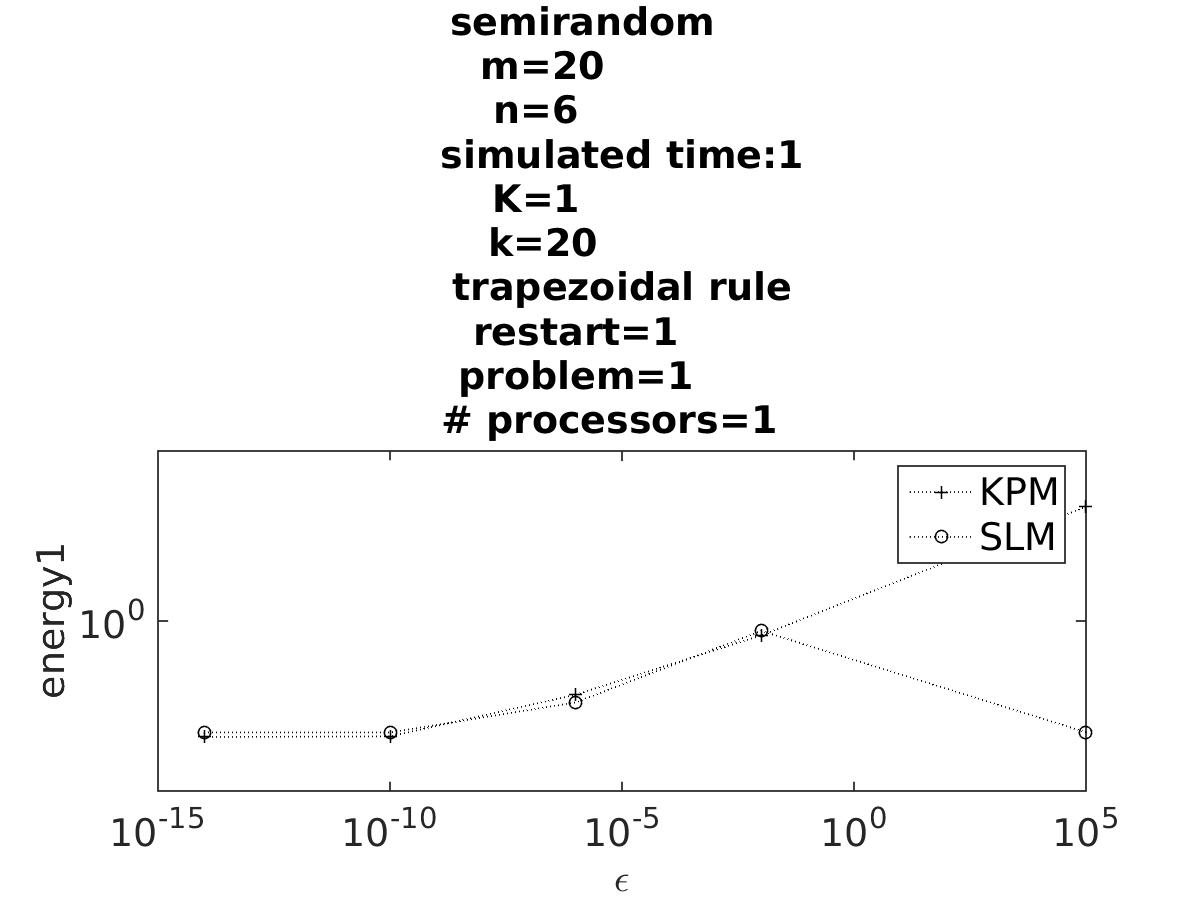
\includegraphics[width=\textwidth]{../MATLAB/fig/compareEnergy.jpg}
                \caption{ The difference in energy with and without restart. }
                \label{fig:compareEnergy}
        \end{subfigure}
        ~
        \begin{subfigure}[b]{0.3\textwidth}
                \includegraphics[width=\textwidth]{../MATLAB/fig/compareError.jpg}
                \caption{ The difference in error with and without restart. }
                \label{fig:compareEnergy}
        \end{subfigure}
        ~
        \begin{subfigure}[b]{0.3\textwidth}
                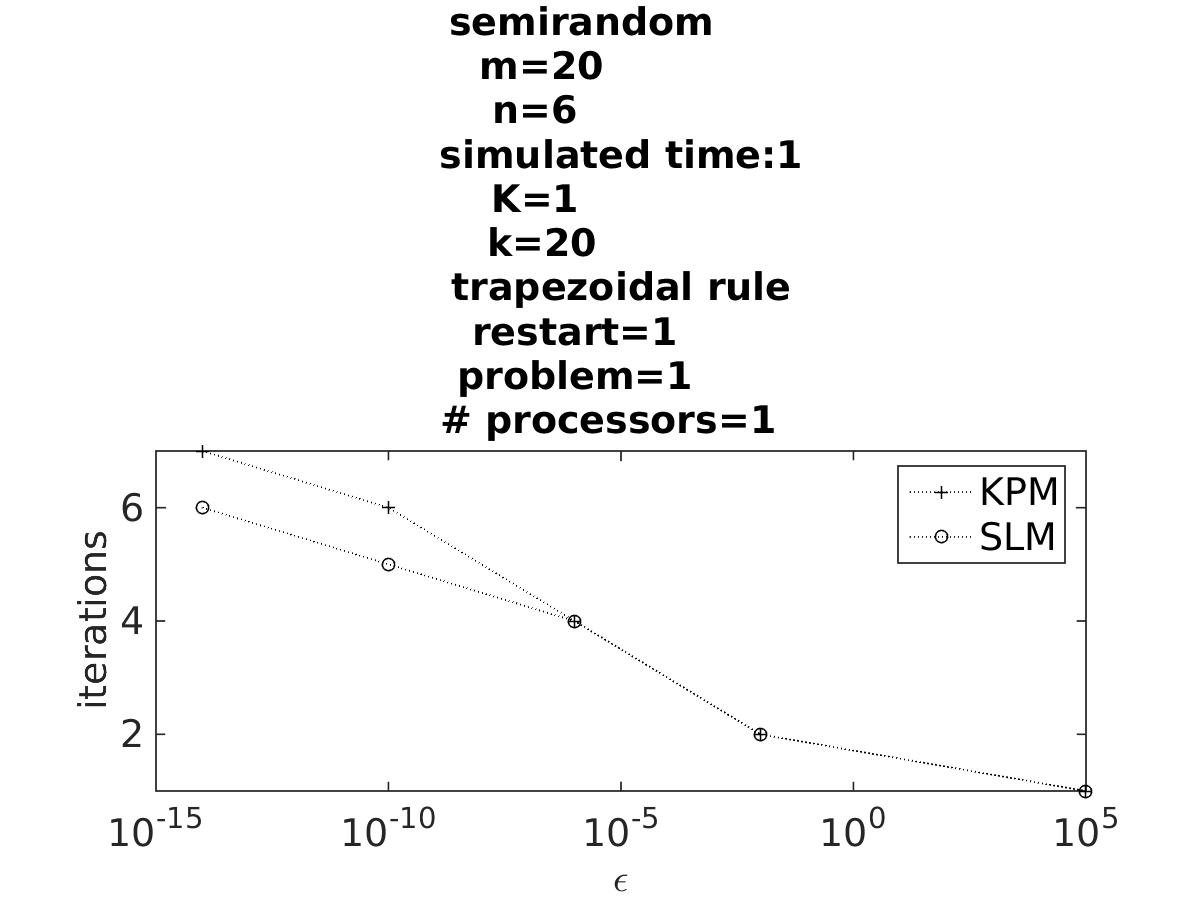
\includegraphics[width=\textwidth]{../MATLAB/fig/compareIter.jpg}
                \caption{ The number of iterations performed with and without restarting.  }
                \label{fig:compareIter}
        \end{subfigure}
        \caption{ The figure shows how the different methods change the energy with and without restarting.  }
        \label{fig:compare}
\end{figure}
!!!!!!!!!!!!!!!!!!!!!!!!!!!!!!NY tekst her!!!!!!!!!!!!!!!!!!!!!!!!\\

\begin{figure}[H]
        \centering
        \begin{subfigure}[b]{0.3\textwidth}
                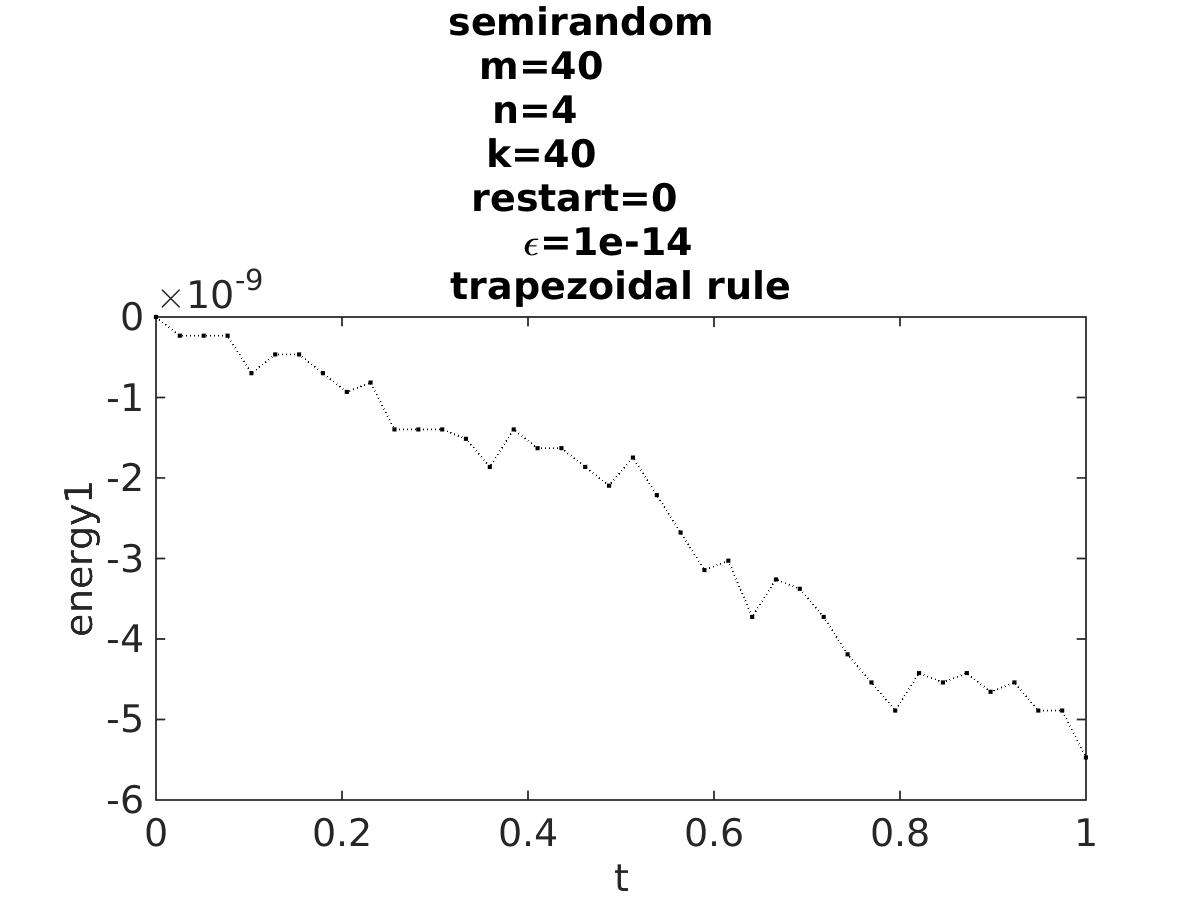
\includegraphics[width=\textwidth]{../MATLAB/fig/energytestrestart0.jpg}
                \caption{ Without restart. }
                \label{fig:energytestrestart0}
        \end{subfigure}
        ~
        \begin{subfigure}[b]{0.3\textwidth}
                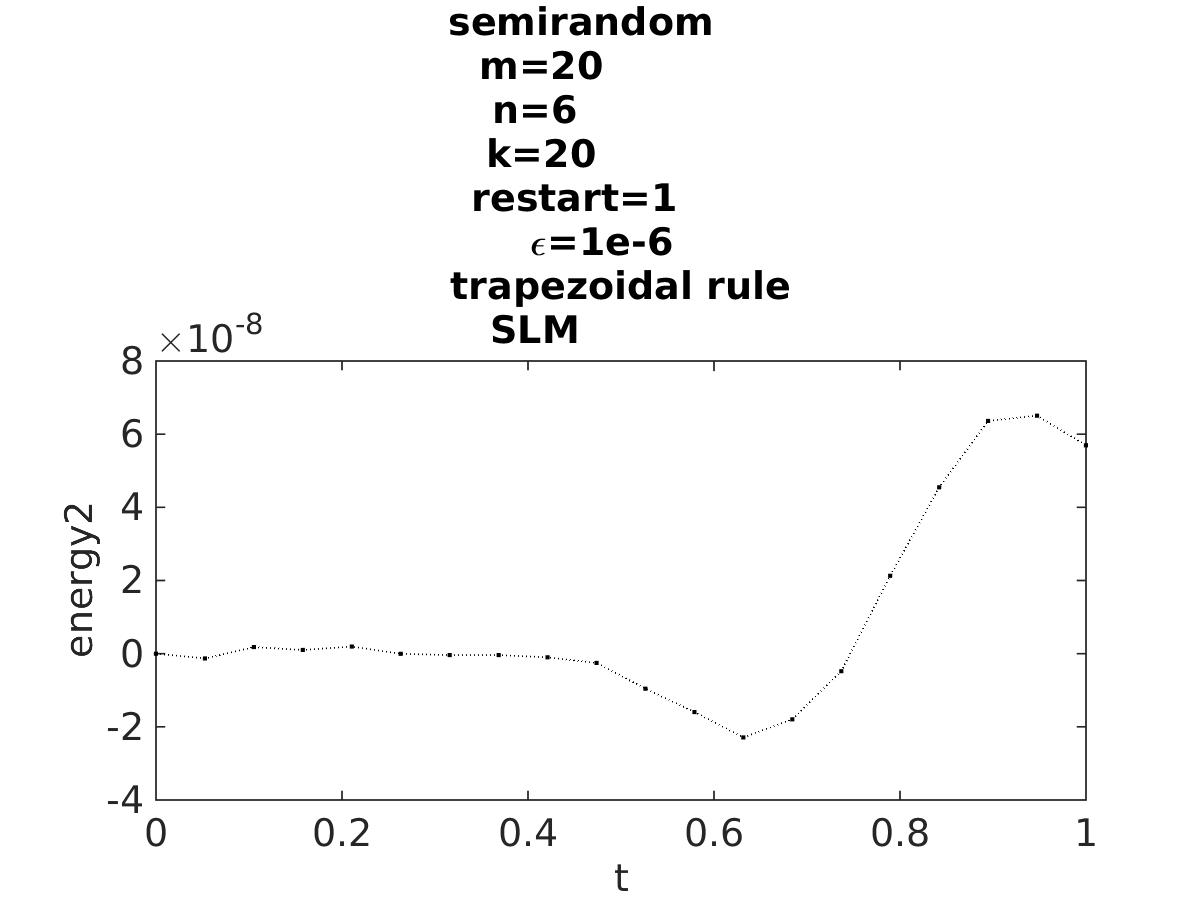
\includegraphics[width=\textwidth]{../MATLAB/fig/energytestrestart2.jpg}
                \caption{ With restart, the number of iterations $= x$ }
                \label{fig:energytestrestart2}
        \end{subfigure}
        ~
		\begin{subfigure}[b]{0.3\textwidth}
                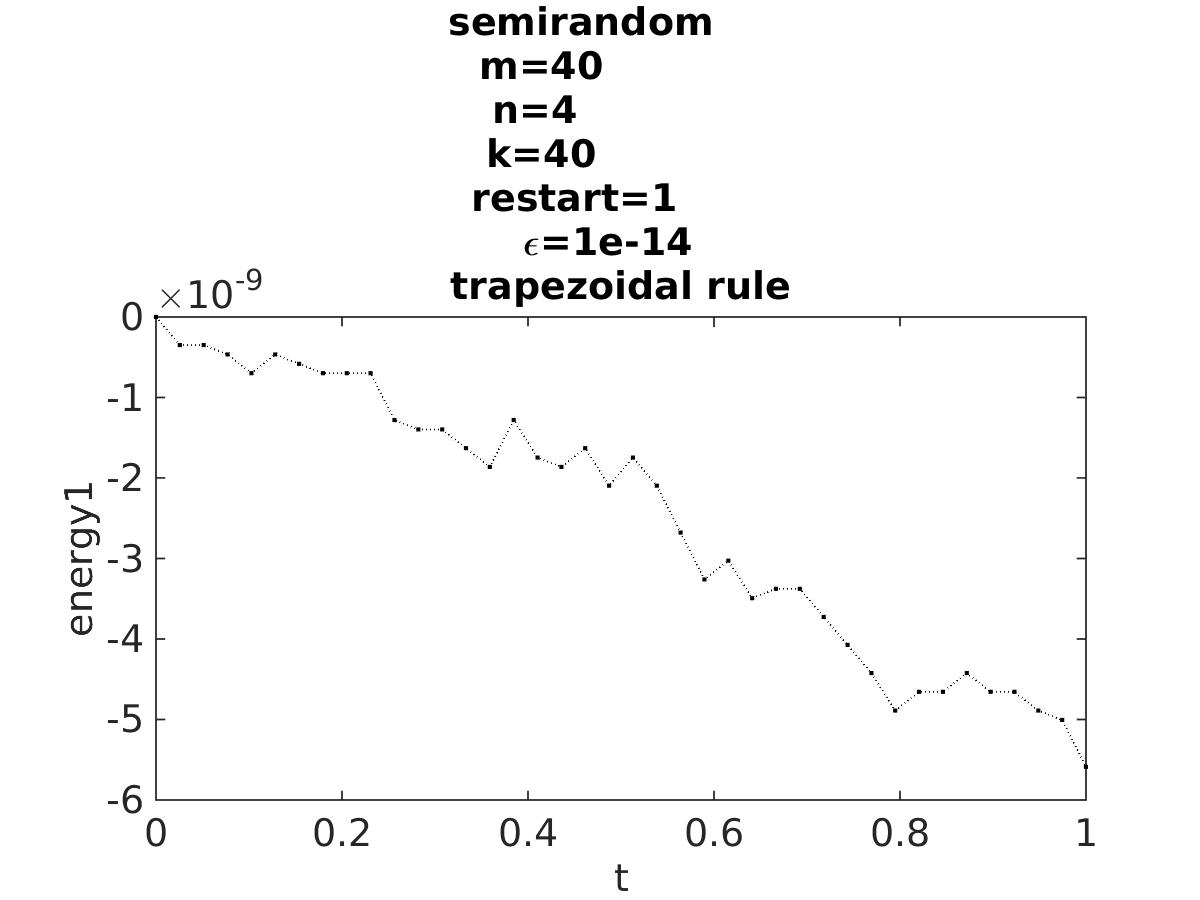
\includegraphics[width=\textwidth]{../MATLAB/fig/energytestrestart1.jpg}
                \caption{ With restart, the number of iterations $= 10$ }
                \label{fig:energytestrestart1}
        \end{subfigure}
        
        \begin{subfigure}[b]{0.3\textwidth}
                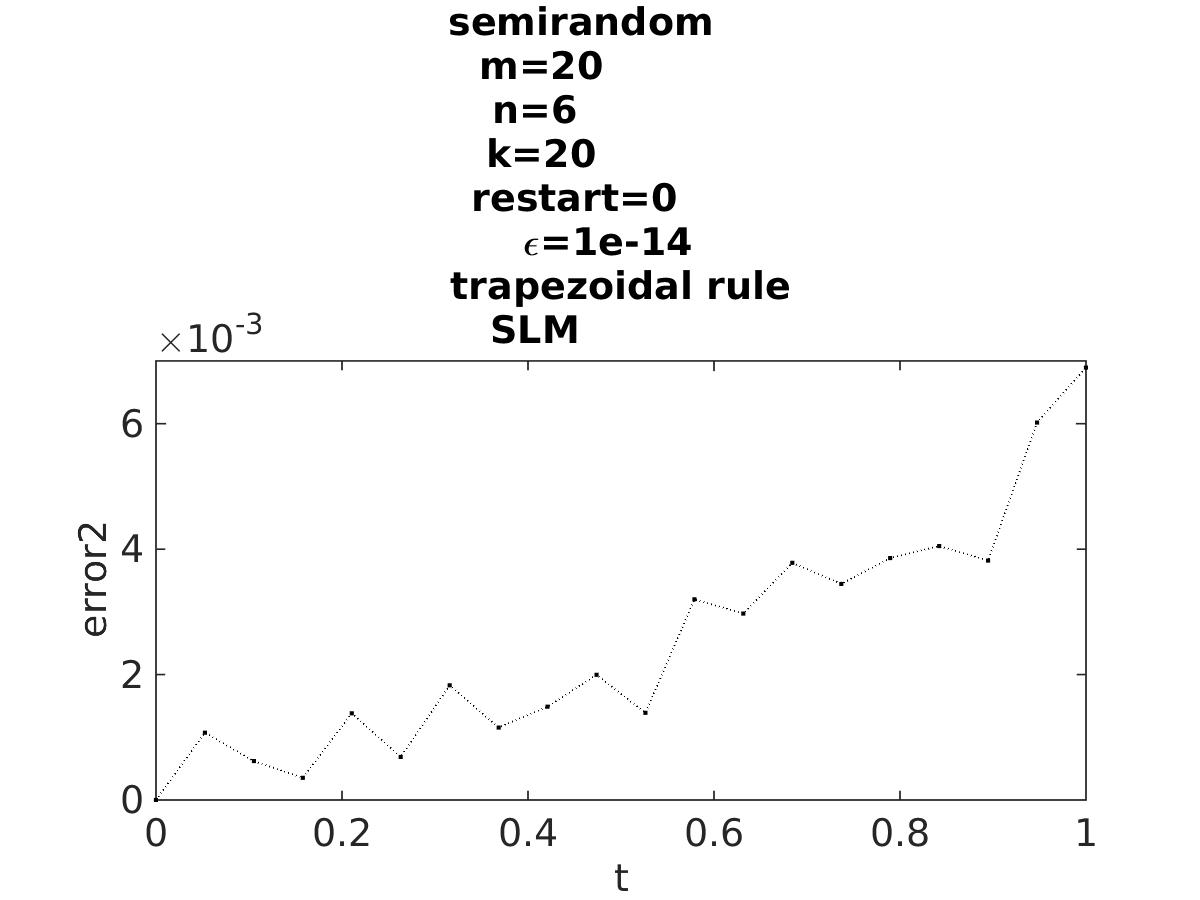
\includegraphics[width=\textwidth]{../MATLAB/fig/errortestrestart0.jpg}
                \caption{ Without restart. }
                \label{fig:energytestrestart0}
        \end{subfigure}
        ~
        \begin{subfigure}[b]{0.3\textwidth}
                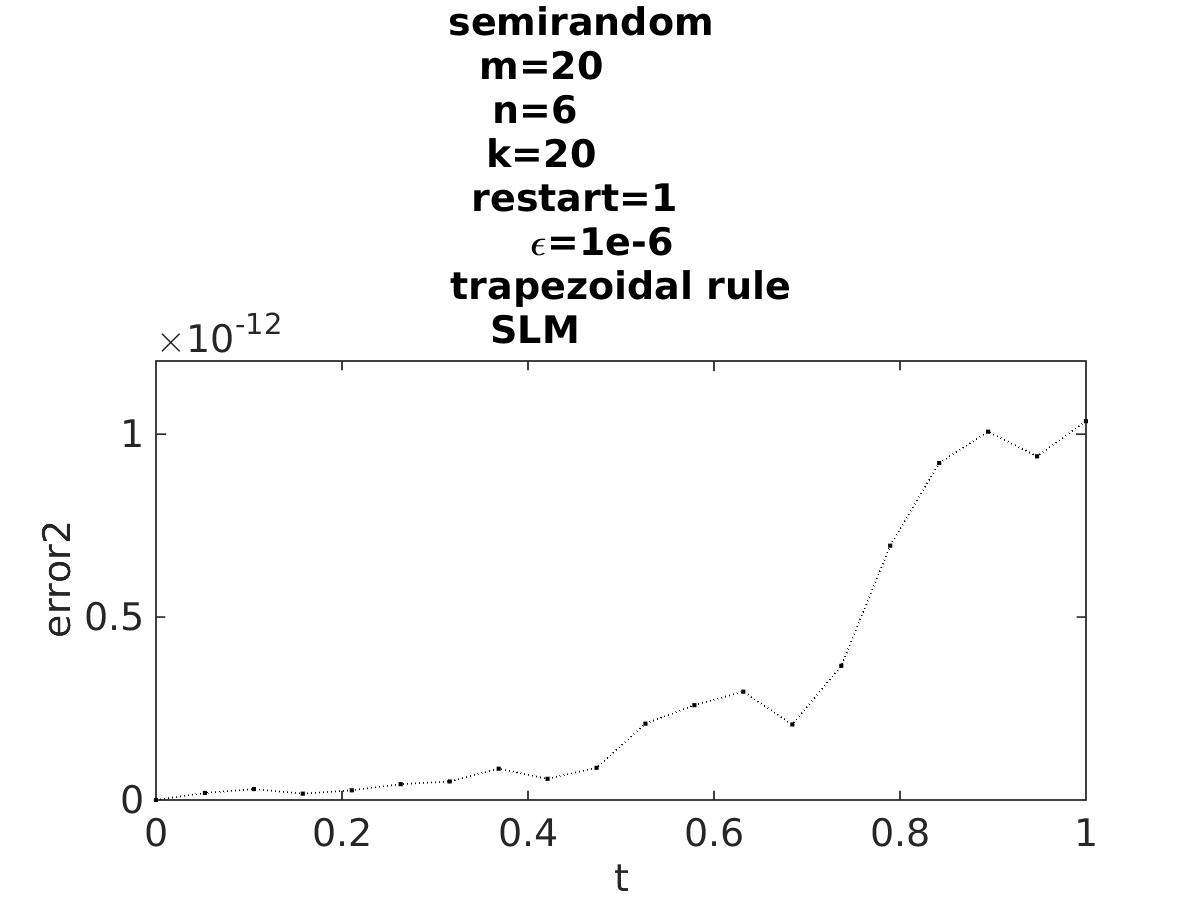
\includegraphics[width=\textwidth]{../MATLAB/fig/errortestrestart2.jpg}
                \caption{ With restart, the number of iterations $= x$ }
                \label{fig:energytestrestart2}
        \end{subfigure}
        ~
        \begin{subfigure}[b]{0.3\textwidth}
                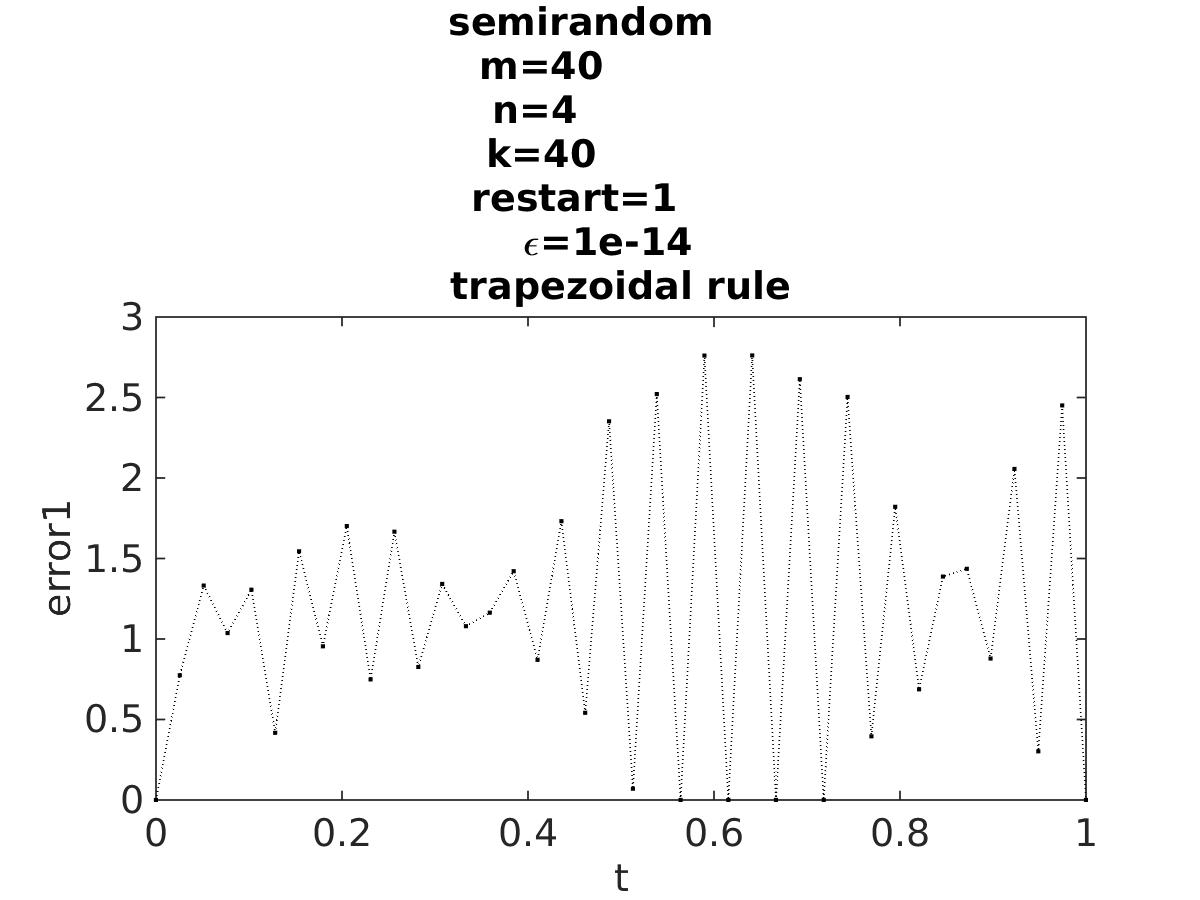
\includegraphics[width=\textwidth]{../MATLAB/fig/errortestrestart1.jpg}
                \caption{ With restart, the number of iterations $= 10$ }
                \label{fig:energytestrestart1}
        \end{subfigure}
        
        
        \caption{ The figures shows the change in energy over time.}
        \label{fig:energytestrestart}
\end{figure}
The figure above shows very little change in energy with SLM, with and without several restarts. \\

The figures below shows the same as figure \ref{fig:energytestrestart}, but with KPM instead of SLM. 

\begin{figure}[H]
        \centering
        \begin{subfigure}[b]{0.3\textwidth}
                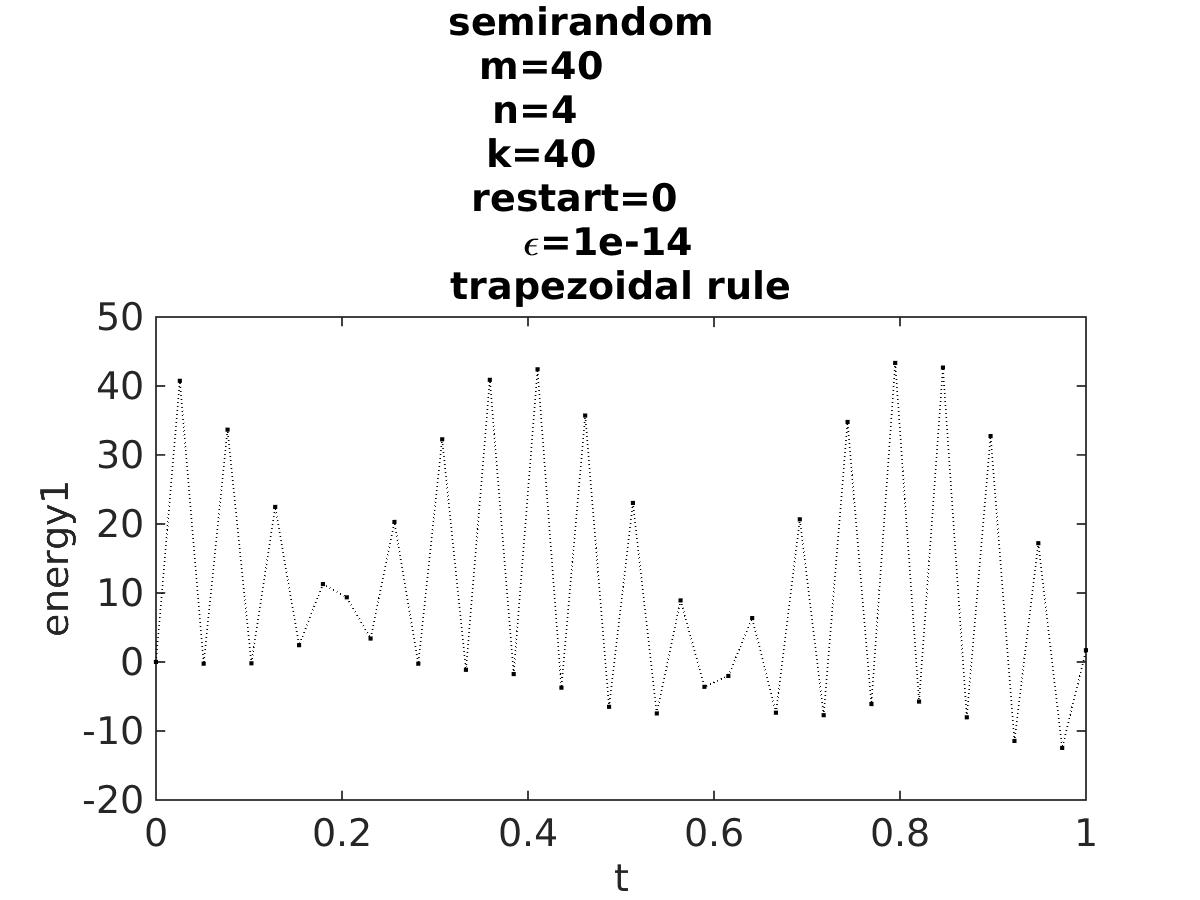
\includegraphics[width=\textwidth]{../MATLAB/fig/energyarnrestart0.jpg}
                \caption{  Without restart. }
                \label{fig:energyarnrestart0}
        \end{subfigure}%
        ~
        \begin{subfigure}[b]{0.3\textwidth}
                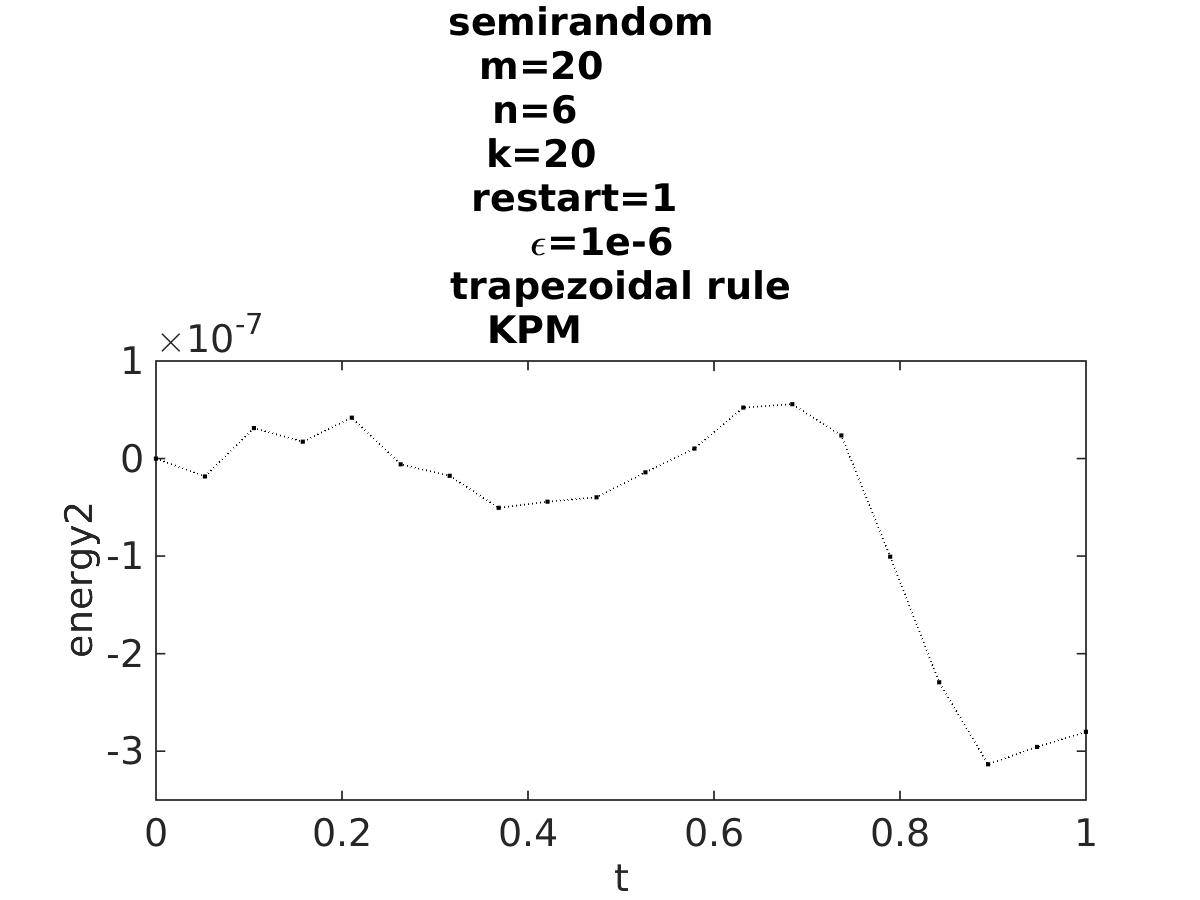
\includegraphics[width=\textwidth]{../MATLAB/fig/energyarnrestart2.jpg}
                \caption{ With restart, the number of iterations $ = 4$ }
                \label{fig:energyarnrestart2}
        \end{subfigure}
        ~
        \begin{subfigure}[b]{0.3\textwidth}
                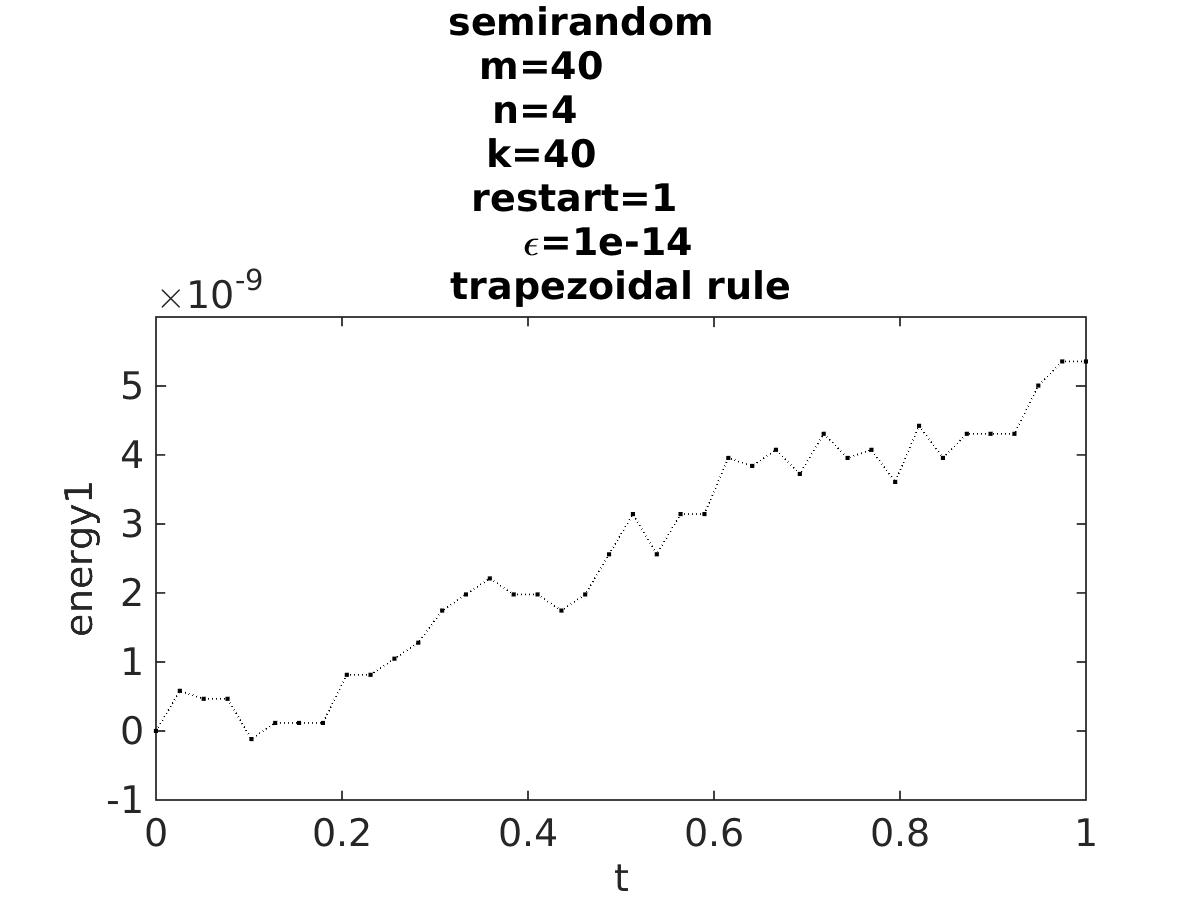
\includegraphics[width=\textwidth]{../MATLAB/fig/energyarnrestart1.jpg}
                \caption{ With restart, the number of iterations $ = 11$ }
                \label{fig:energyarnrestart1}
        \end{subfigure}
        
        \begin{subfigure}[b]{0.3\textwidth}
                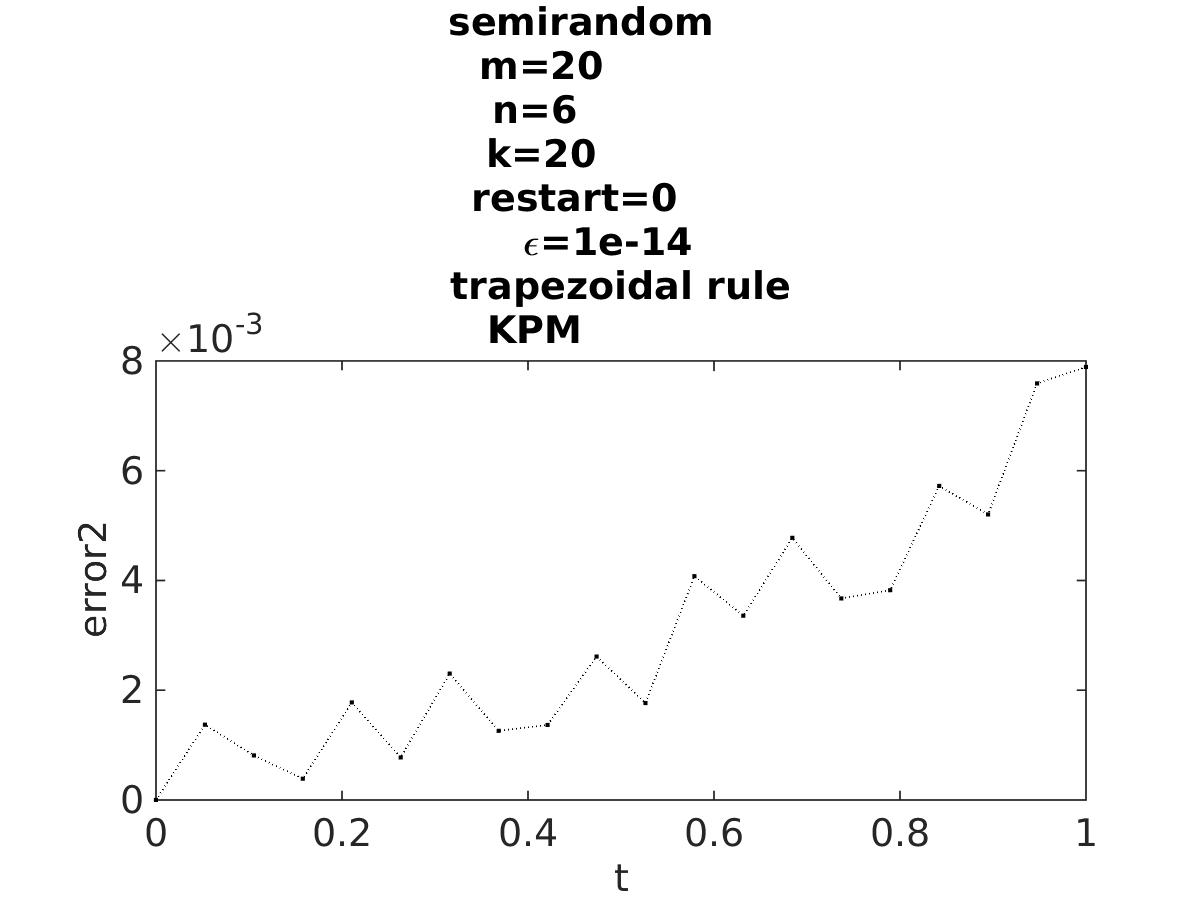
\includegraphics[width=\textwidth]{../MATLAB/fig/errorarnrestart0.jpg}
                \caption{  Without restart. }
                \label{fig:energyarnrestart0}
        \end{subfigure}%
        ~
        \begin{subfigure}[b]{0.3\textwidth}
                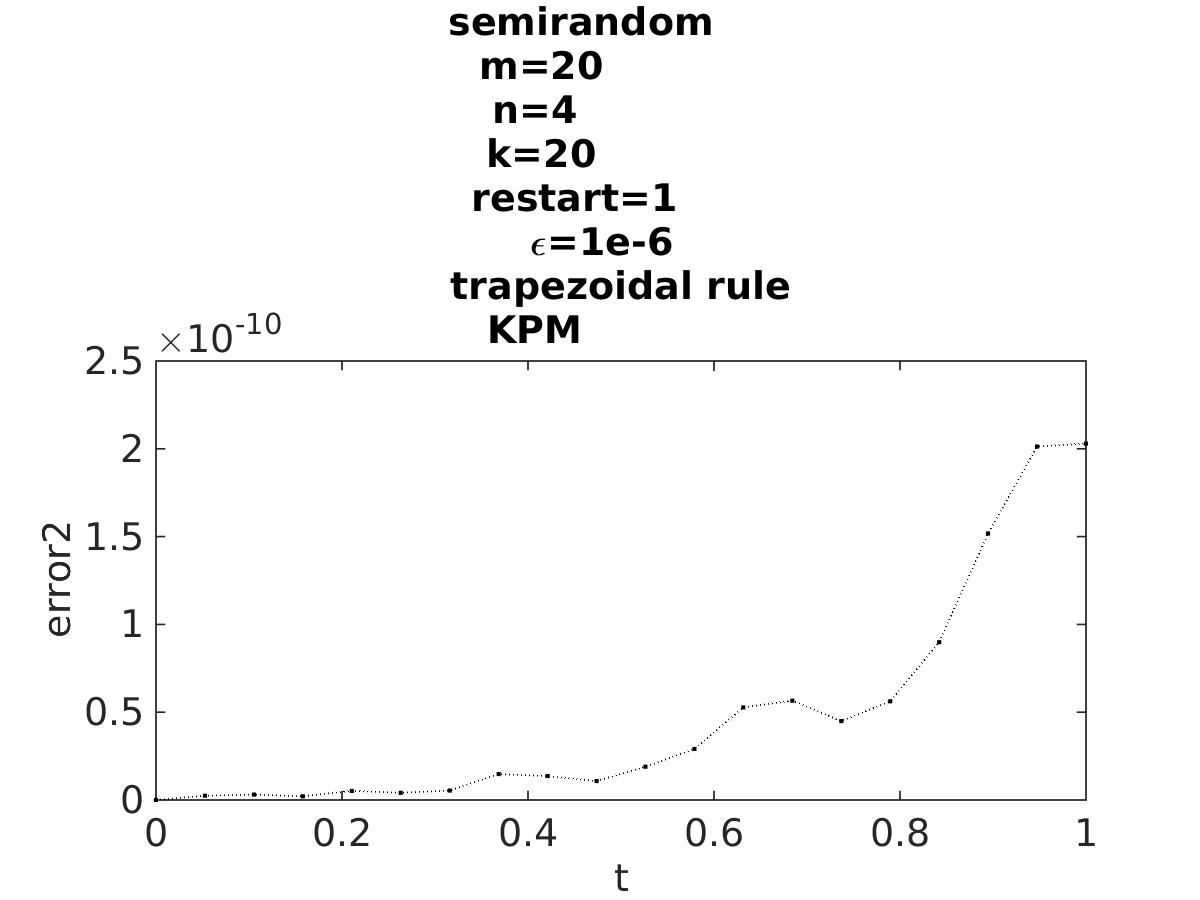
\includegraphics[width=\textwidth]{../MATLAB/fig/errorarnrestart2.jpg}
                \caption{ With restart, the number of iterations $ = 4$ }
                \label{fig:energyarnrestart2}
        \end{subfigure}
        ~
        \begin{subfigure}[b]{0.3\textwidth}
                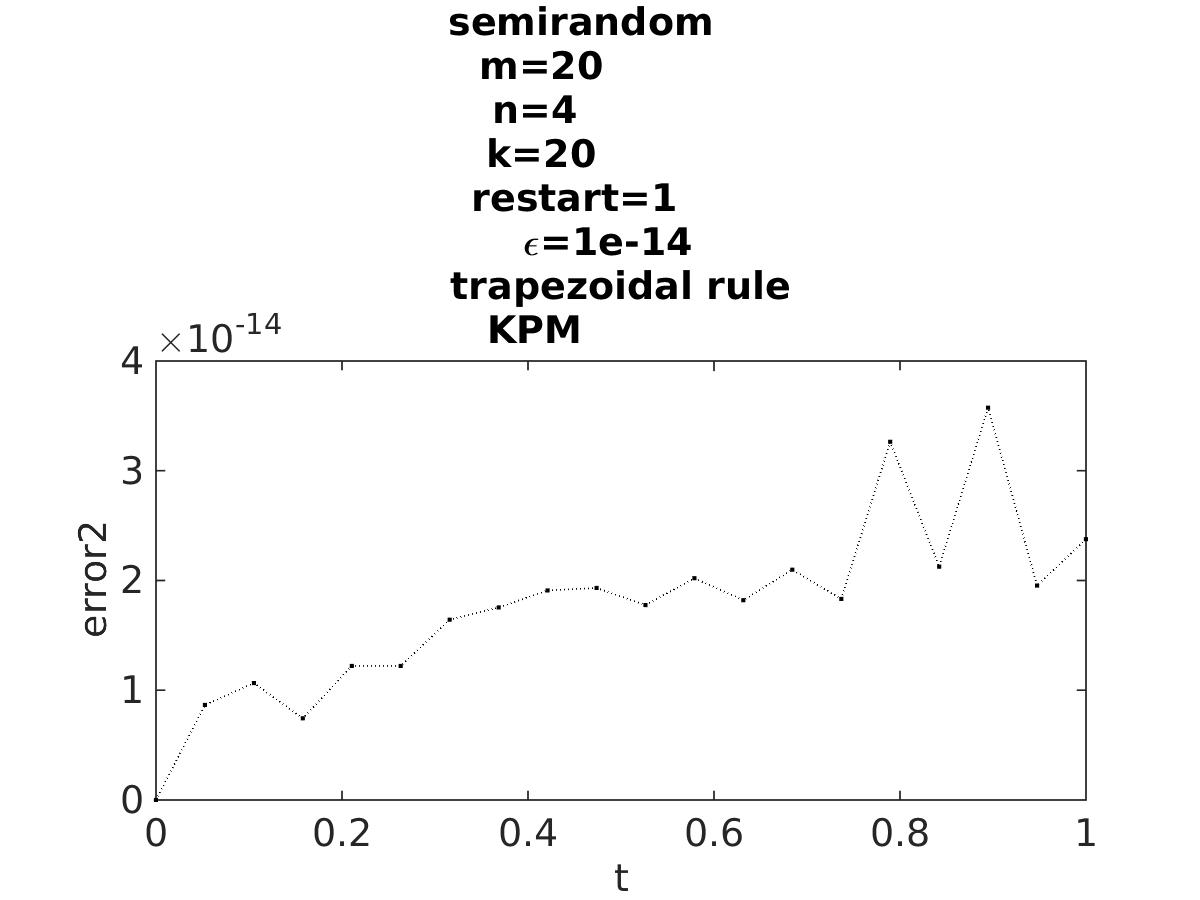
\includegraphics[width=\textwidth]{../MATLAB/fig/errorarnrestart1.jpg}
                \caption{ With restart, the number of iterations $ = 11$ }
                \label{fig:energyarnrestart1}
        \end{subfigure}
        \caption{ Figures showing the change in energy over time. }
        \label{fig:energyarnrestart}
\end{figure}

When comparing figure \ref{fig:energytestrestart0} and \ref{fig:energytestrestart1} it becomes clear that SLM's does not alter the energy significantly when performing the restart. Figure \ref{fig:energyarnrestart0} and \ref{fig:energyarnrestart1} shows that this is not the case for KPM.\\

%!!!!!!!!!!!!!!!!Burde jeg gjøre det samme for feilen?(JA)!!!!!!!!!!!!!!!!!!!!!!!!!!!!!!!\\

%!!!!!!!!!!!!!!!!!!!!!!!ER dette overbevisende nok?!!!!!!!!!!!!!!!!!!!!!!!!!!!!!\\
\section{Varying energy}
!!!!!!!!!!!!!!!!!!Figurene her fungerer ikke!!!!!!!!!!!!!!!!!!!!!!!\\
%\begin{figure}
%	\centering
%	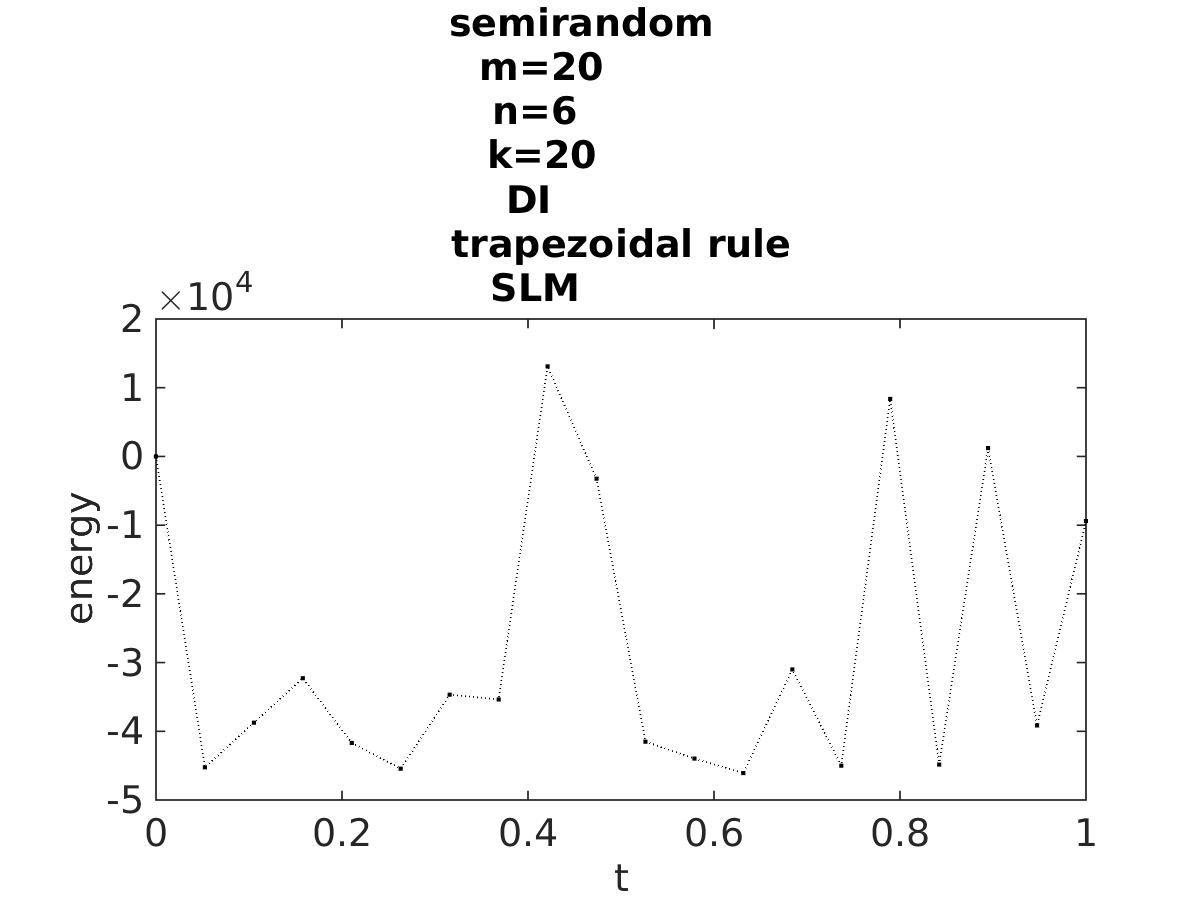
\includegraphics[width=0.45 \textwidth]{../MATLAB/fig/semirandomenergy2.jpg}
%	\caption{!!!!!!!!!!!SKRIV NOE HER!!!!!!!!!!!!!}
%	\label{fig:semirandomenergy1}
%\end{figure}

%\begin{table}
%\centering
%\begin{tabular}{l l l}
%\texttt{restart} & Arnoldi & SLM  \\
%0 & 0.008206143327698 & 0.004387334709463 \\
%1 & 0.000000000058208 & 0.000000000014552 \\
%Iterations & 7 & 6 \\
%\end{tabular}
%\caption{!!!!!!!!!!!!!!!!SKRIV NOE!!!!!!!!!!!!!!!!\\!!!!!!!!Formater tallene penere!!!!!!!!}
%\label{tab:SLMVE}
%\end{table}

\begin{figure}[H]
        \centering
        \begin{subfigure}[b]{0.3\textwidth}
                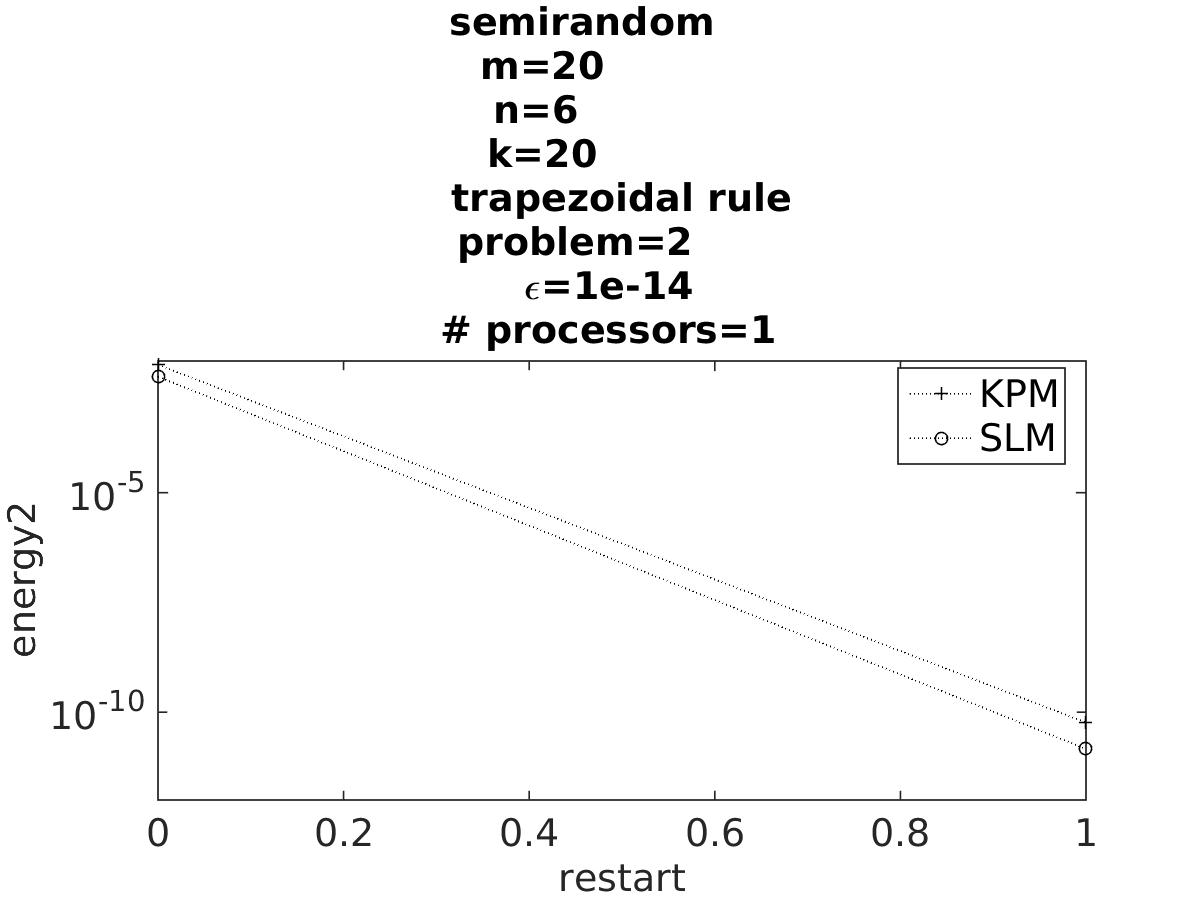
\includegraphics[width=\textwidth]{../MATLAB/fig/compareEnergy2.jpg}
                \caption{ The difference in energy with and without restart. }
                \label{fig:compareEnergy}
        \end{subfigure}
        ~
        \begin{subfigure}[b]{0.3\textwidth}
                \includegraphics[width=\textwidth]{../MATLAB/fig/compareError2.jpg}
                \caption{ The difference in energy with and without restart. }
                \label{fig:compareEnergy}
        \end{subfigure}
        ~
        \begin{subfigure}[b]{0.3\textwidth}
                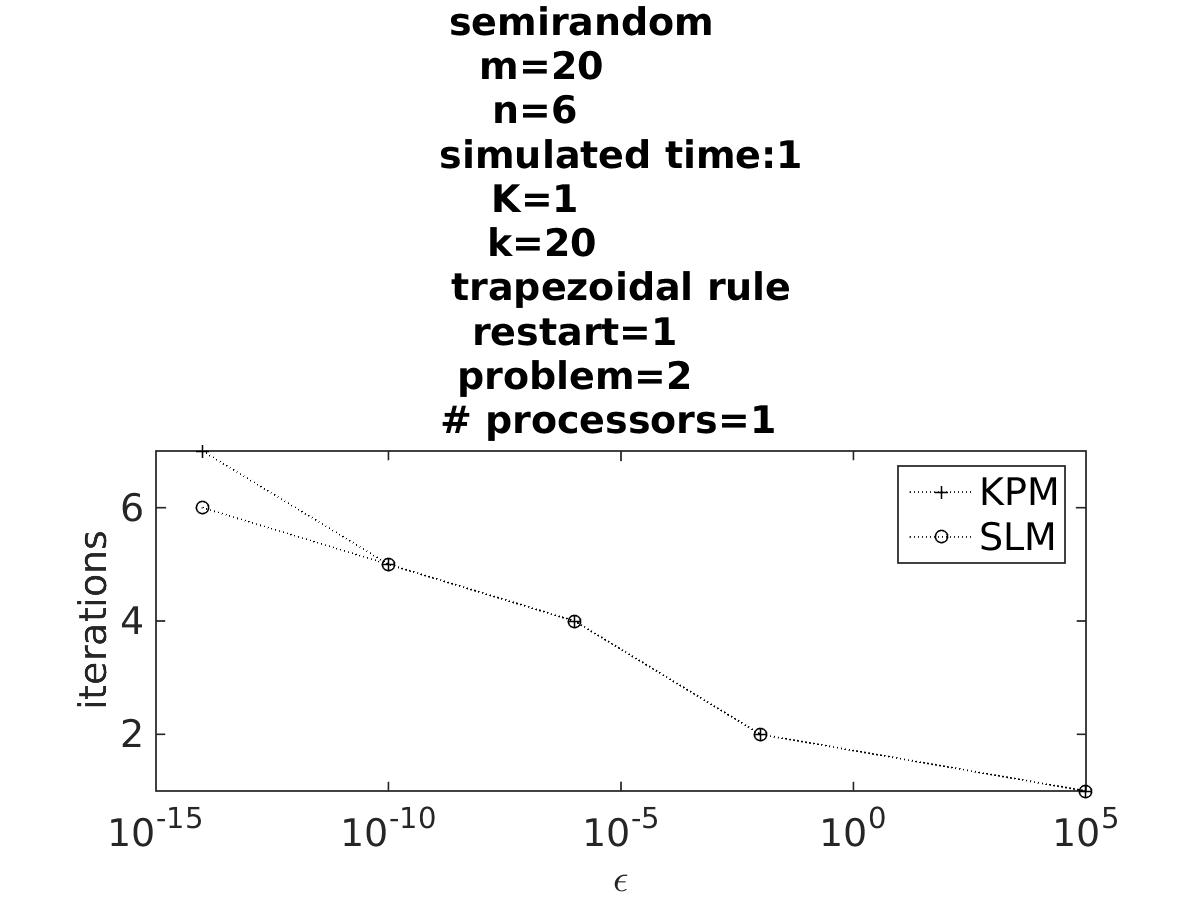
\includegraphics[width=\textwidth]{../MATLAB/fig/compareIter2.jpg}
                \caption{ The number of iterations performed with and without restarting.  }
                \label{fig:compareIter}
        \end{subfigure}
        \caption{ The figure shows how the different methods change the energy with and without restarting.  }
        \label{fig:compare}
\end{figure}

The figures above implies that restarting the SLM does indeed not change the energy. But for KPM it changes quite a bit. 

\begin{figure}[H]
        \centering
        \begin{subfigure}[b]{0.3\textwidth}
                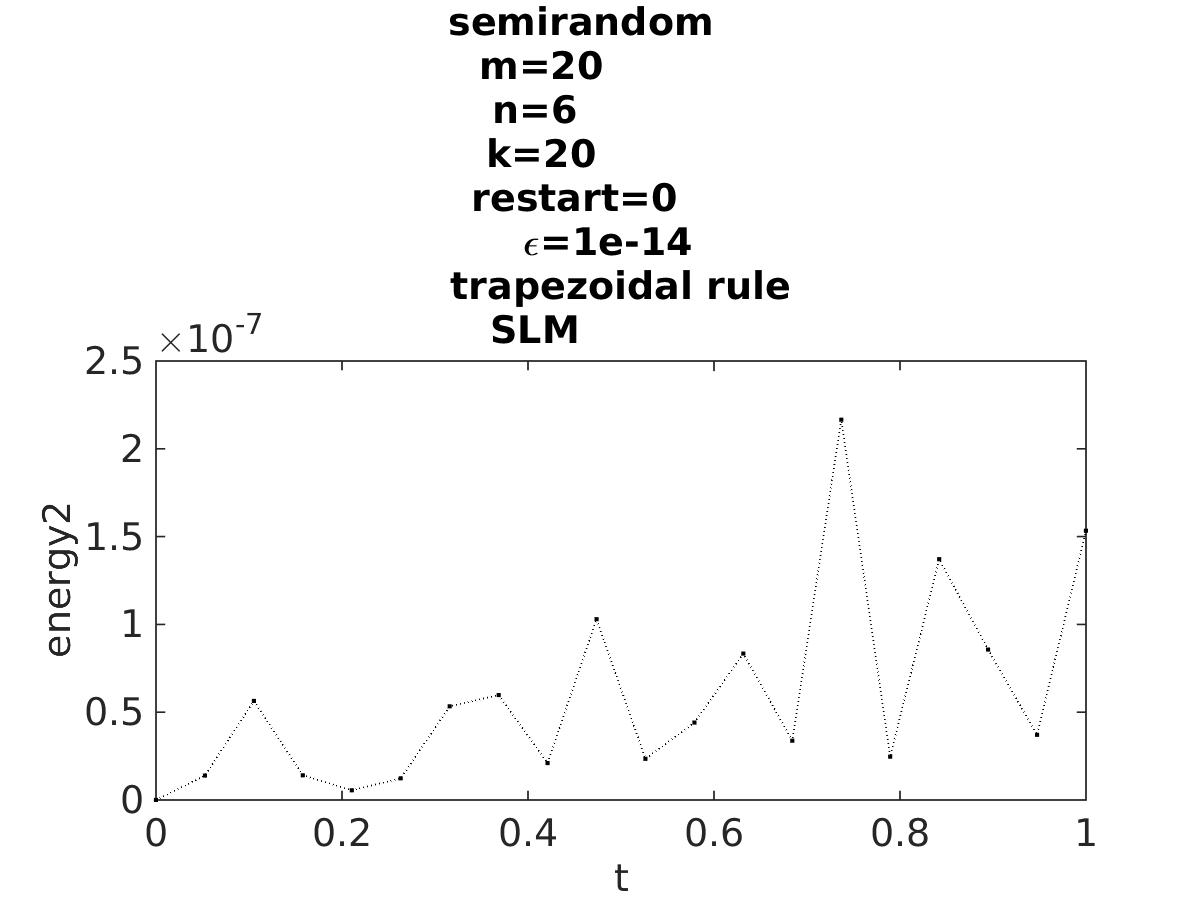
\includegraphics[width=\textwidth]{../MATLAB/fig/energytestrestart02.jpg}
                \caption{ Without restart. }
                \label{fig:energytestrestart02}
        \end{subfigure}
        ~
        \begin{subfigure}[b]{0.3\textwidth}
                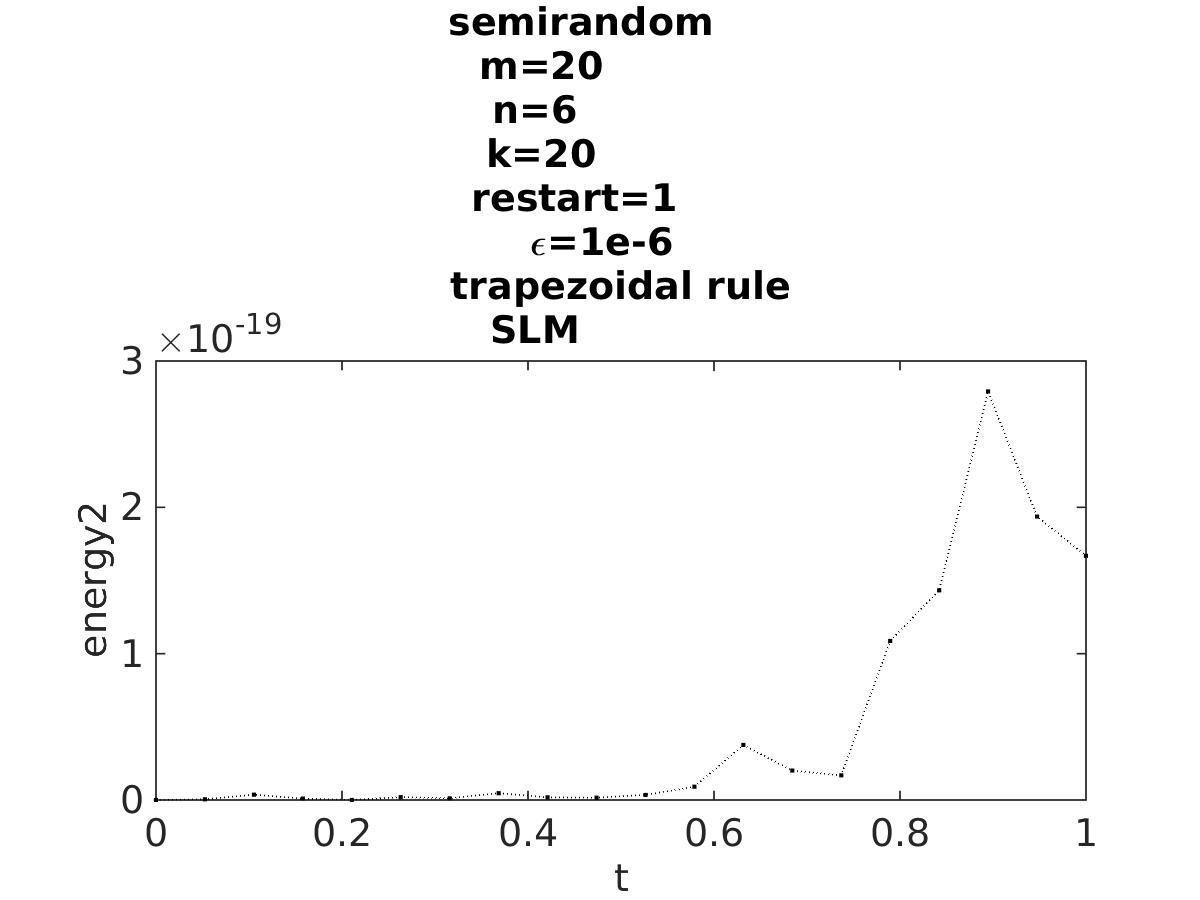
\includegraphics[width=\textwidth]{../MATLAB/fig/energytestrestart22.jpg}
                \caption{ With restart, the number of iterations $= 4$ }
                \label{fig:energytestrestart22}
        \end{subfigure}
        ~
        \begin{subfigure}[b]{0.3\textwidth}
                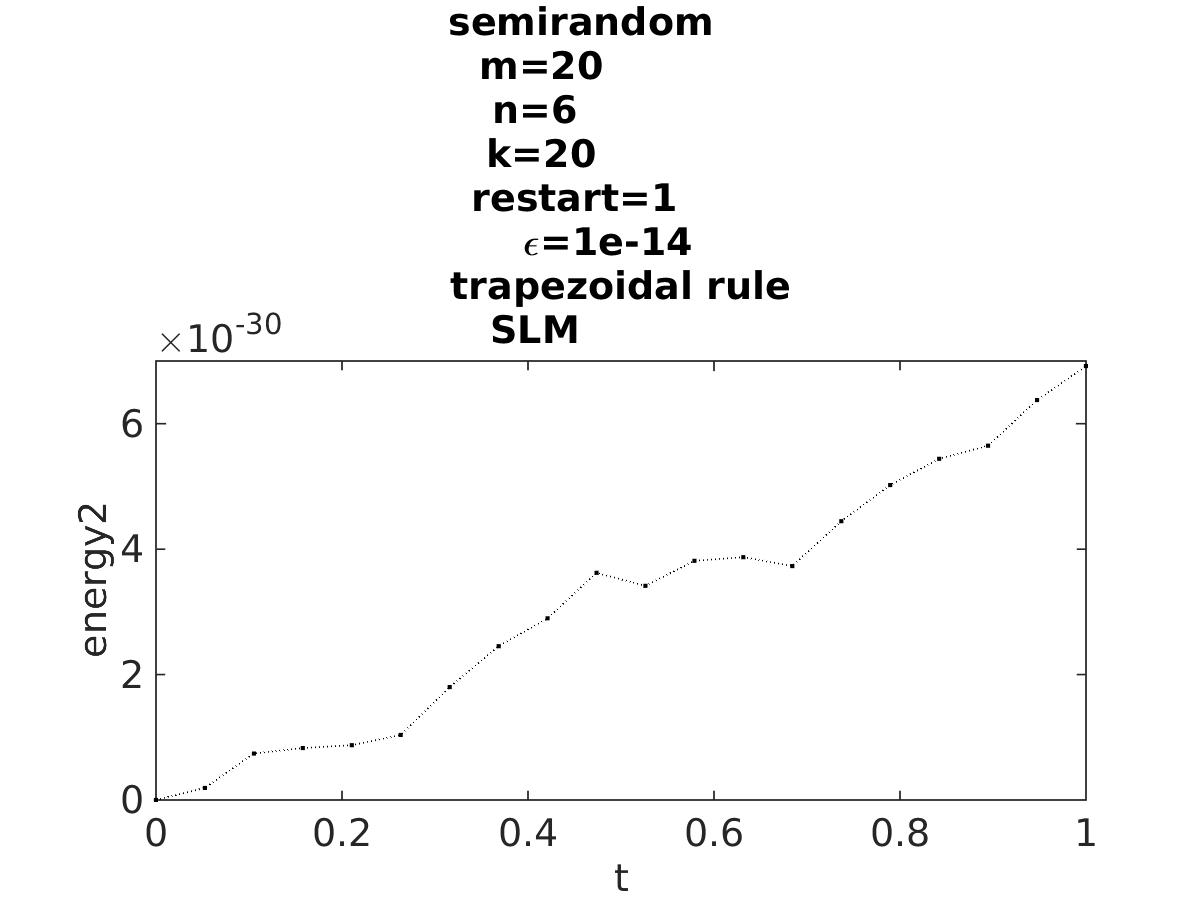
\includegraphics[width=\textwidth]{../MATLAB/fig/energytestrestart12.jpg}
                \caption{ With restart, the number of iterations $= 9$ }
                \label{fig:energytestrestart12}
        \end{subfigure}
        
        \begin{subfigure}[b]{0.3\textwidth}
                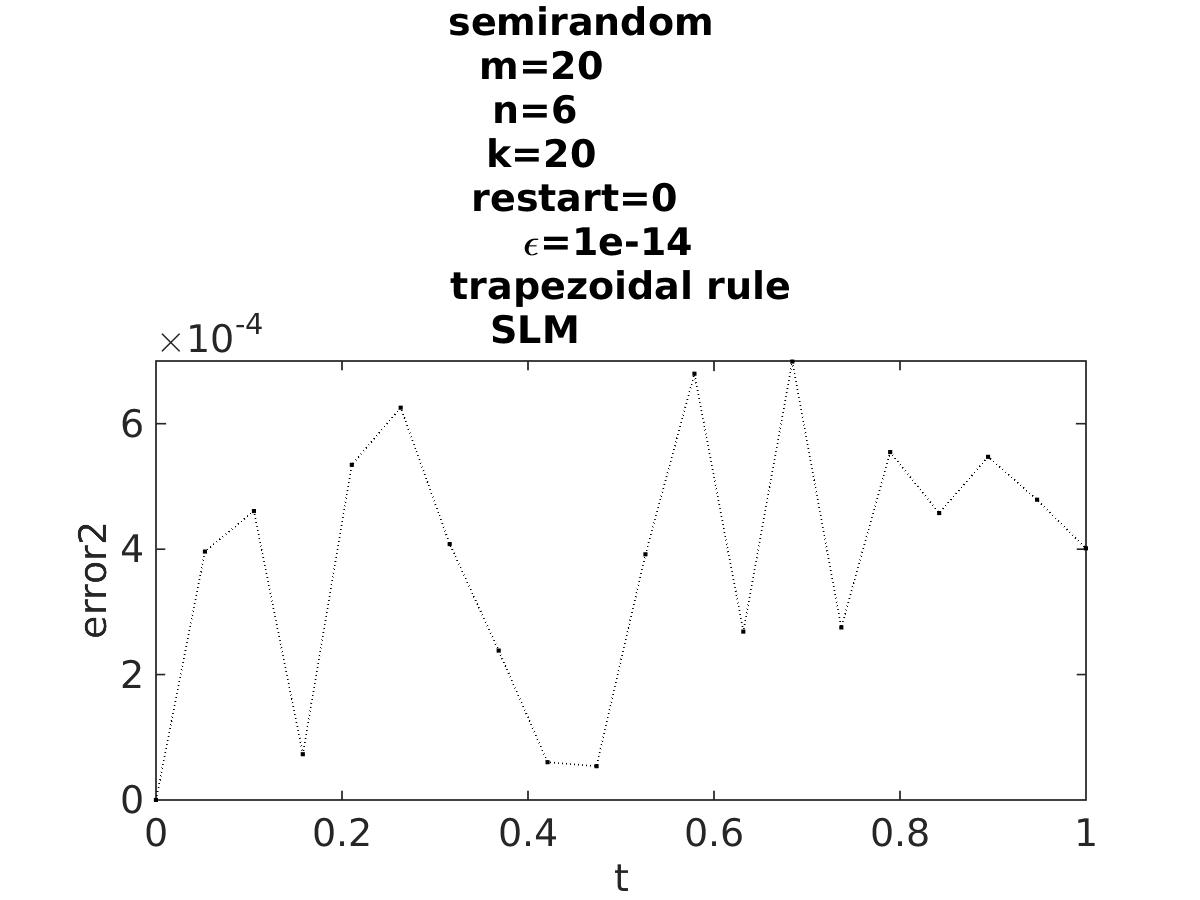
\includegraphics[width=\textwidth]{../MATLAB/fig/errortestrestart02.jpg}
                \caption{ Without restart. }
                \label{fig:energytestrestart02}
        \end{subfigure}
        ~
        \begin{subfigure}[b]{0.3\textwidth}
                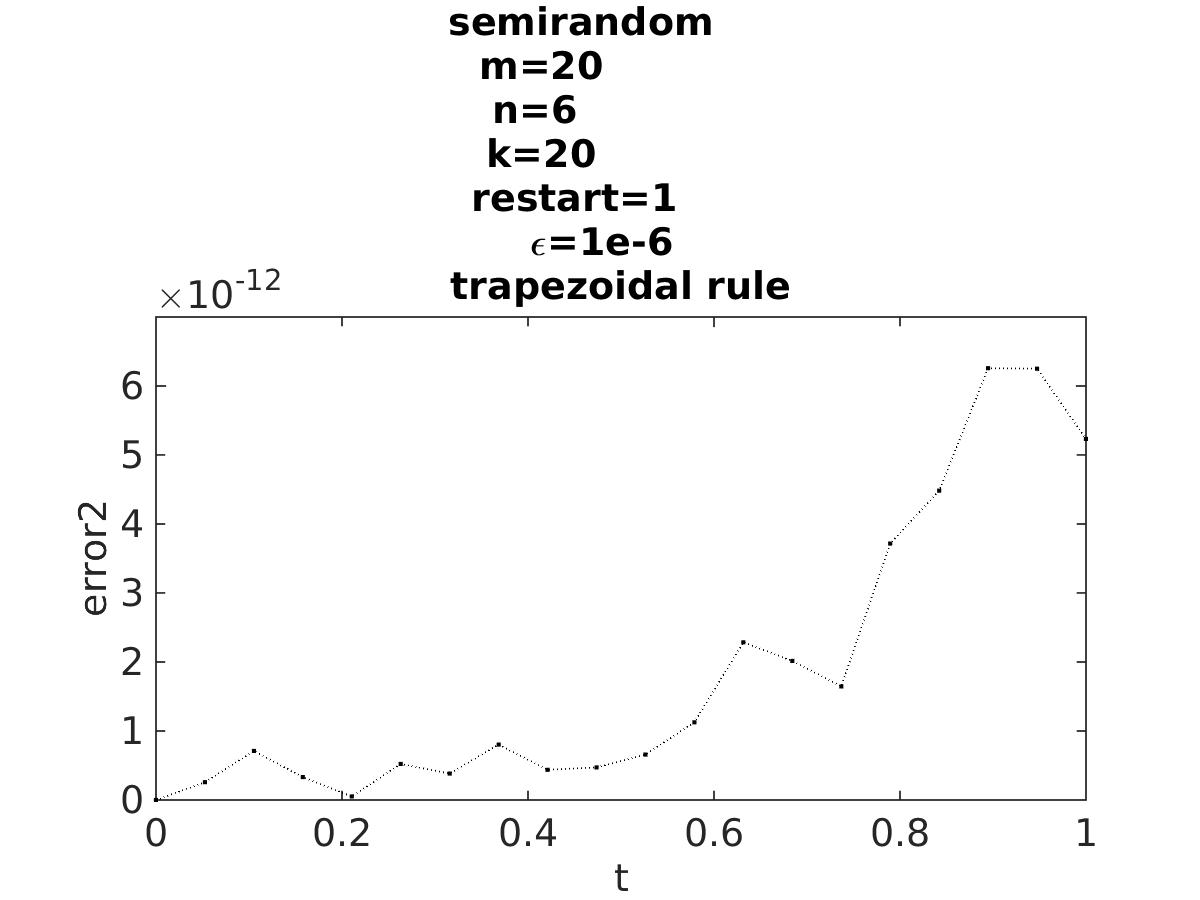
\includegraphics[width=\textwidth]{../MATLAB/fig/errortestrestart22.jpg}
                \caption{ With restart, the number of iterations $= 4$ }
                \label{fig:energytestrestart22}
        \end{subfigure}
        ~
		\begin{subfigure}[b]{0.3\textwidth}
                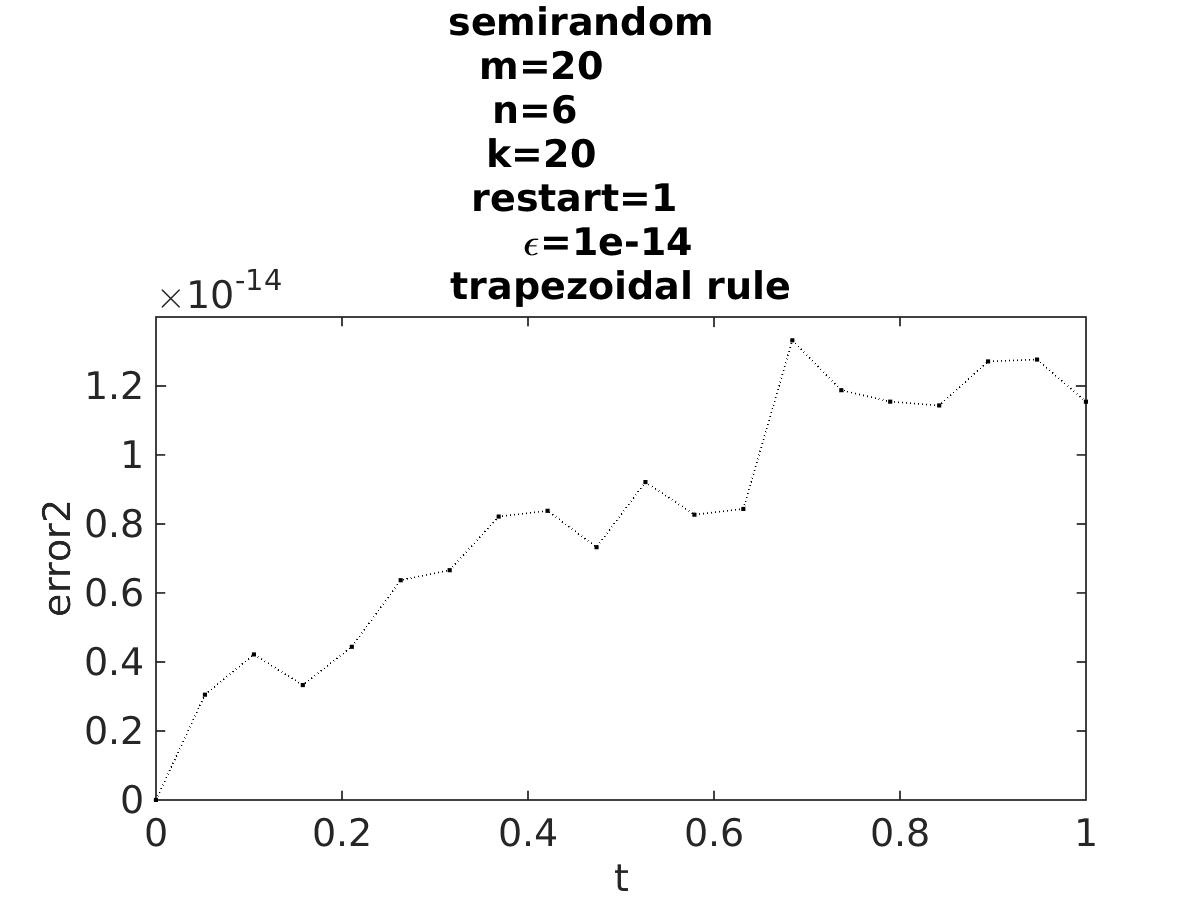
\includegraphics[width=\textwidth]{../MATLAB/fig/errortestrestart12.jpg}
                \caption{ With restart, the number of iterations $= 9$ }
                \label{fig:energytestrestart12}
        \end{subfigure}
        \caption{ The figures shows the change in energy over time.}
        \label{fig:energytestrestart2}
\end{figure}
The figure above shows very little change in energy with SLM, with and without several restarts. \\

The figures below shows the same as figure \ref{fig:energytestrestart2}, but with KPM instead of SLM. 

\begin{figure}[H]
        \centering
        \begin{subfigure}[b]{0.3\textwidth}
                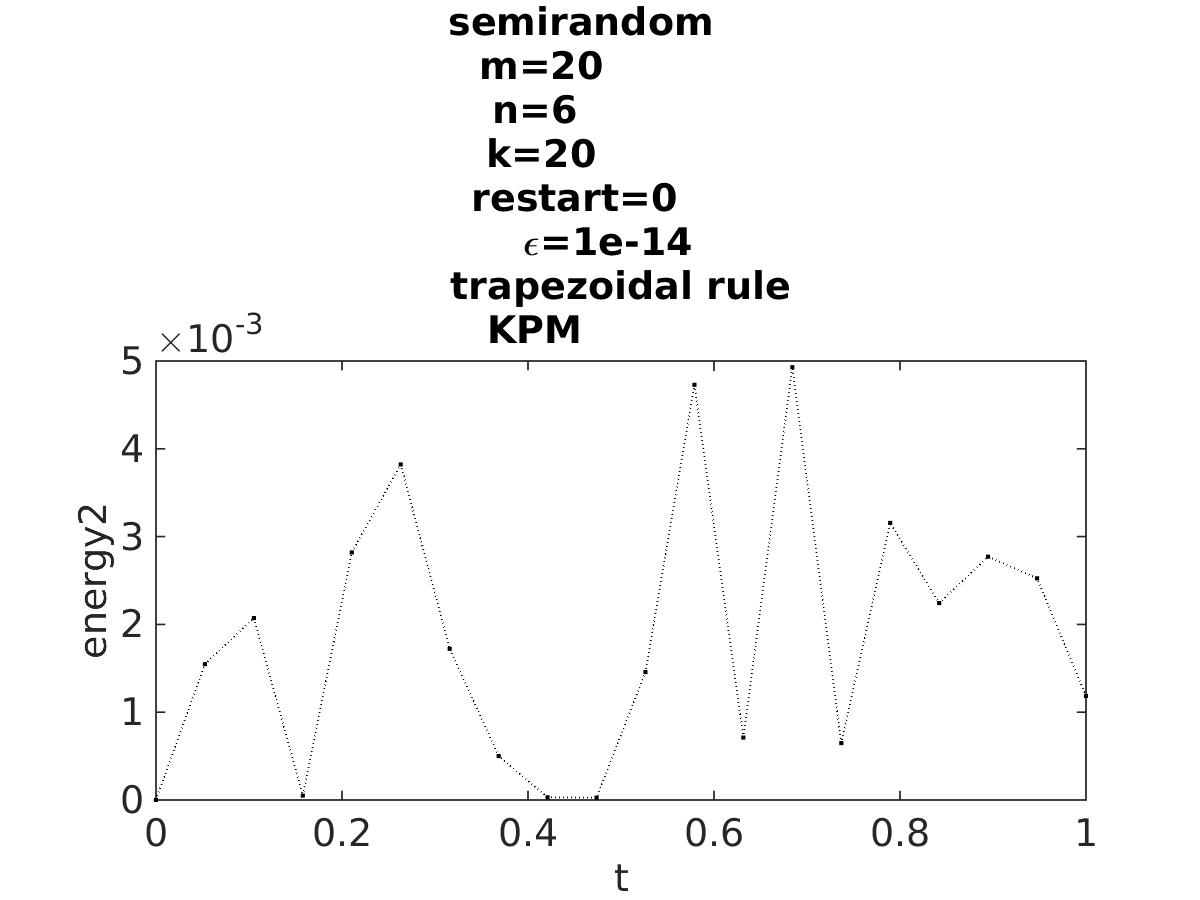
\includegraphics[width=\textwidth]{../MATLAB/fig/energyarnrestart02.jpg}
                \caption{  Without restart. }
                \label{fig:energyarnrestart02}
        \end{subfigure}%
        ~
        \begin{subfigure}[b]{0.3\textwidth}
                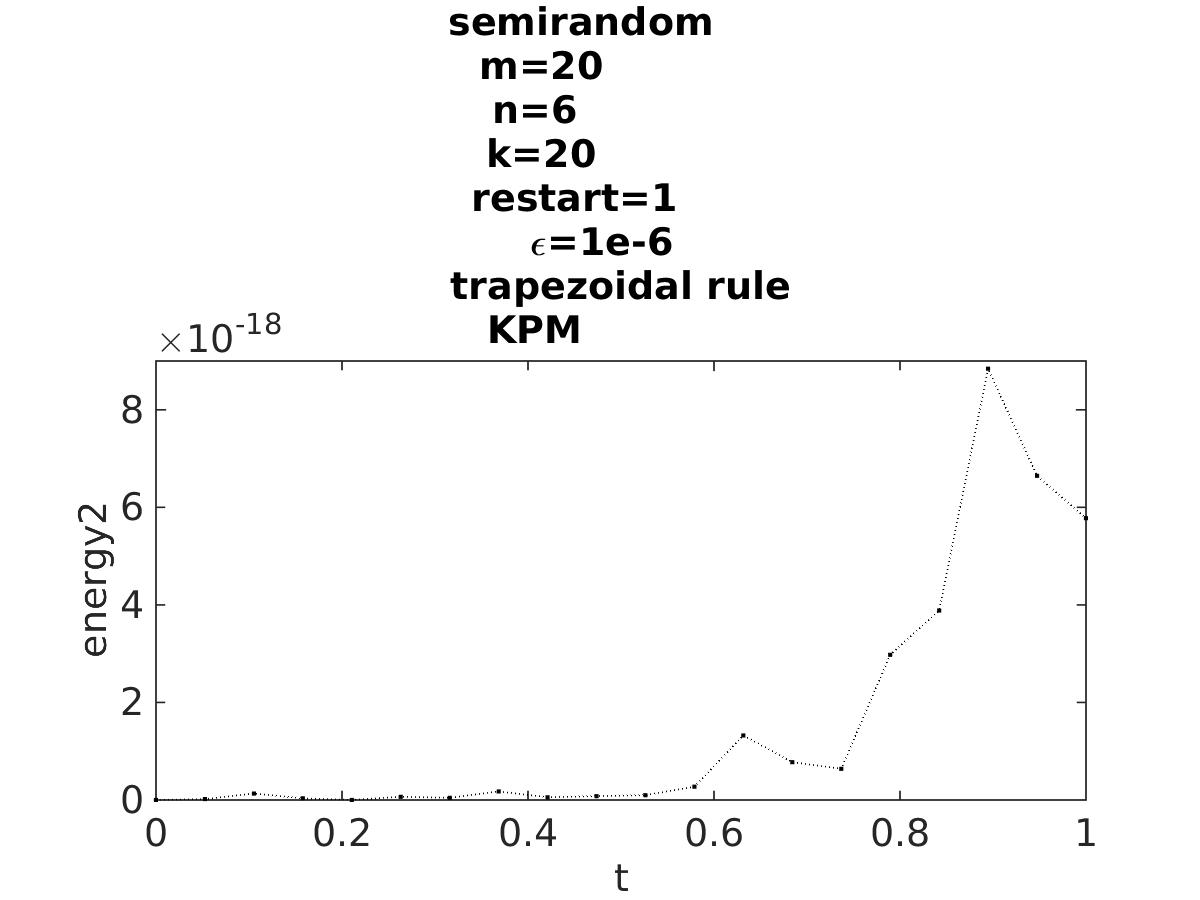
\includegraphics[width=\textwidth]{../MATLAB/fig/energyarnrestart22.jpg}
                \caption{ With restart, the number of iterations $ = 4$ }
                \label{fig:energyarnrestart22}
        \end{subfigure}
        ~
        \begin{subfigure}[b]{0.3\textwidth}
                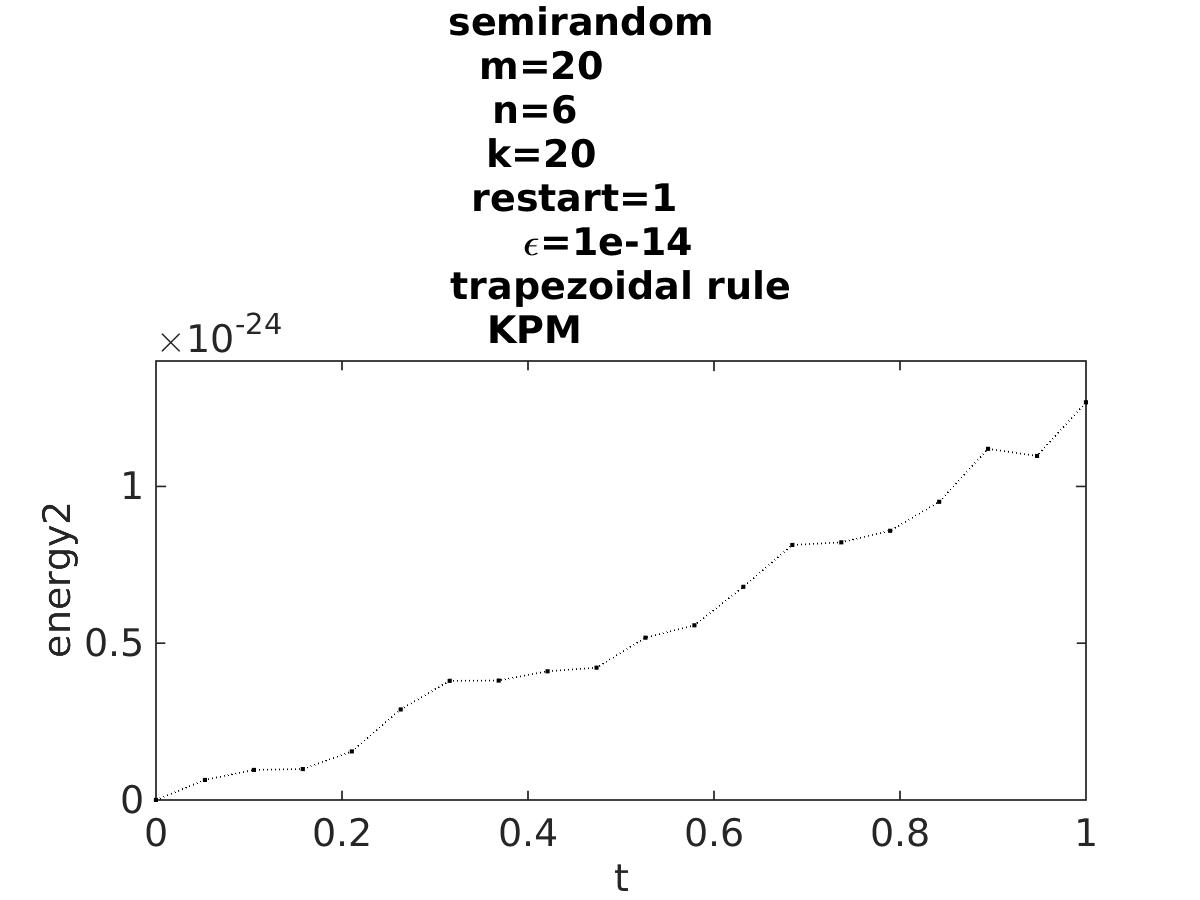
\includegraphics[width=\textwidth]{../MATLAB/fig/energyarnrestart12.jpg}
                \caption{ With restart, the number of iterations $ = 11$ }
                \label{fig:energyarnrestart12}
        \end{subfigure}
        
        \begin{subfigure}[b]{0.3\textwidth}
                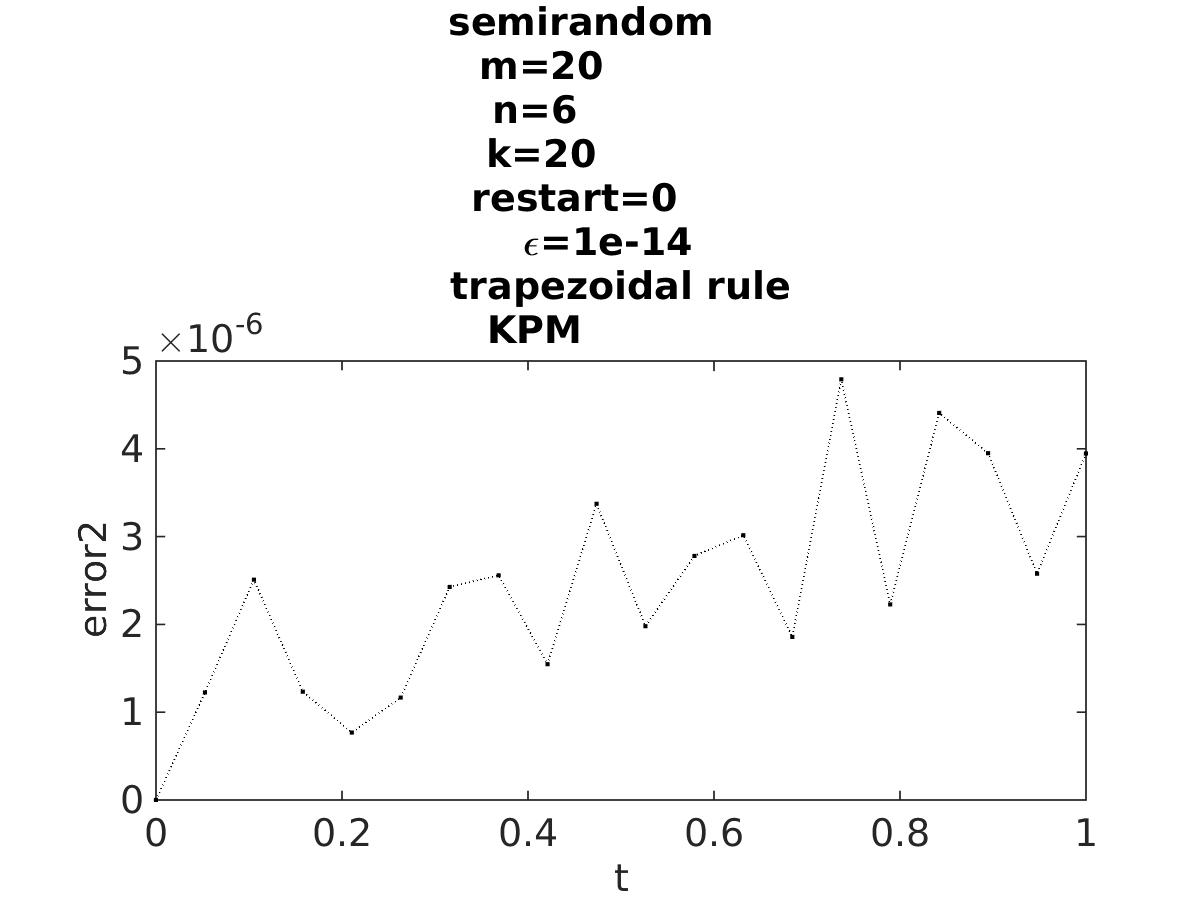
\includegraphics[width=\textwidth]{../MATLAB/fig/errorarnrestart02.jpg}
                \caption{  Without restart. }
                \label{fig:energyarnrestart02}
        \end{subfigure}%
        ~
        \begin{subfigure}[b]{0.3\textwidth}
                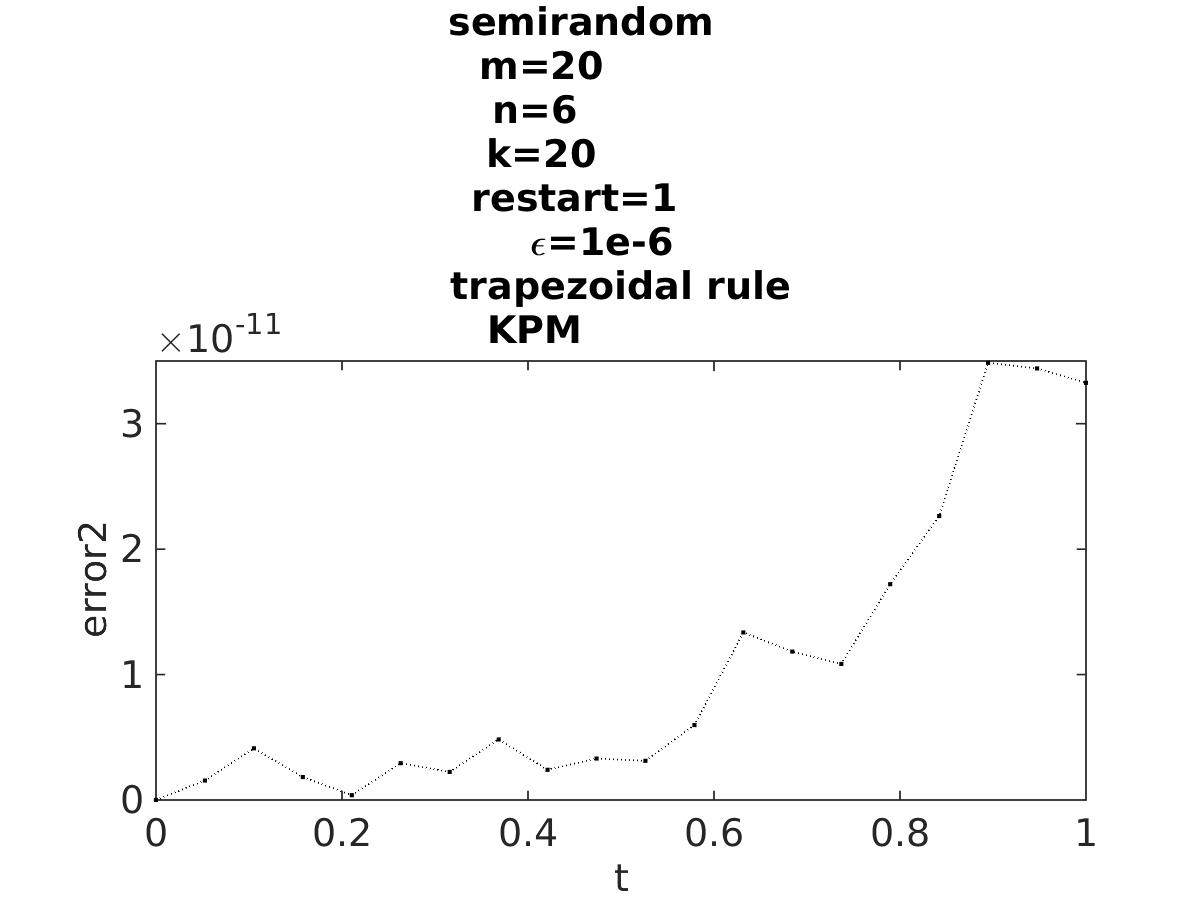
\includegraphics[width=\textwidth]{../MATLAB/fig/errorarnrestart22.jpg}
                \caption{ With restart, the number of iterations $ = 4$ }
                \label{fig:energyarnrestart22}
        \end{subfigure}
        ~
        \begin{subfigure}[b]{0.3\textwidth}
                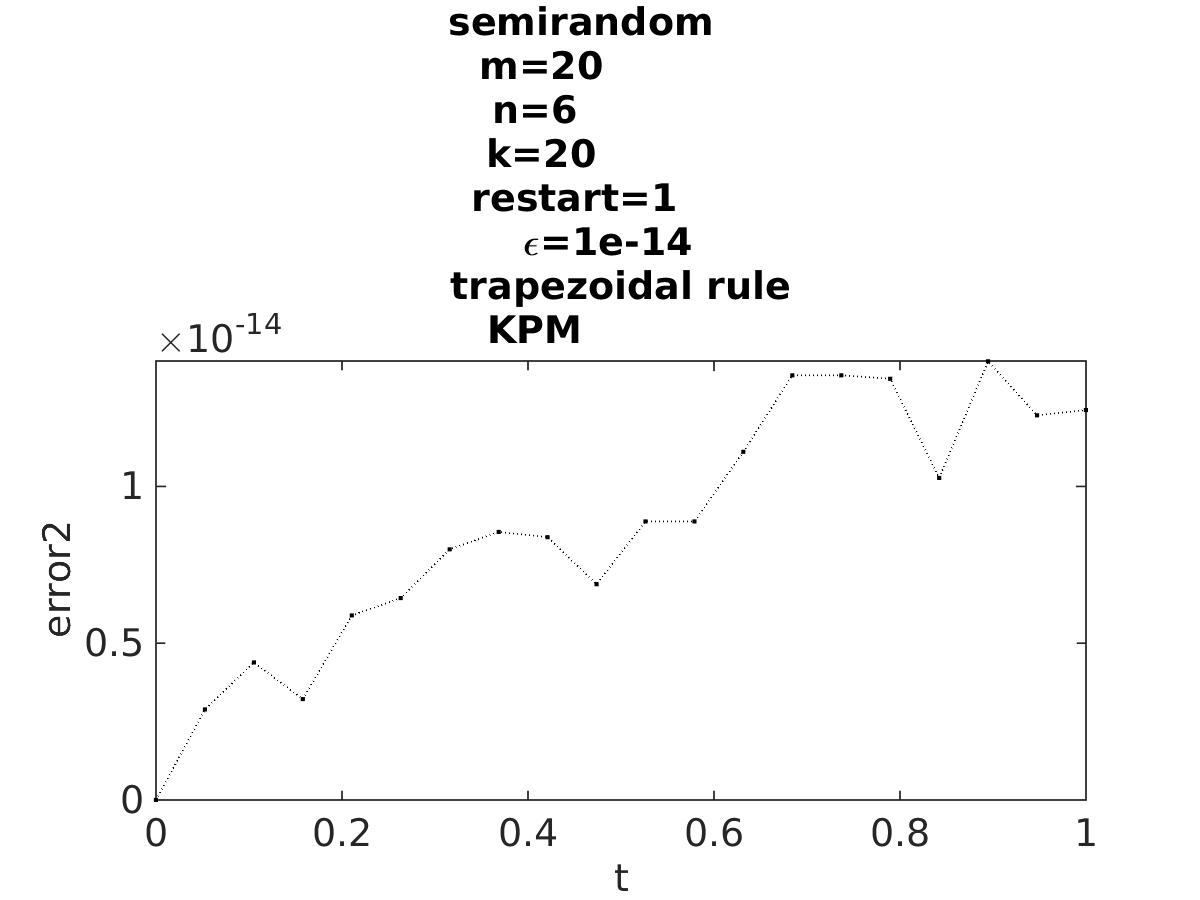
\includegraphics[width=\textwidth]{../MATLAB/fig/errorarnrestart12.jpg}
                \caption{ With restart, the number of iterations $ = 11$ }
                \label{fig:energyarnrestart12}
        \end{subfigure}
        \caption{ Figures showing the change in energy over time. }
        \label{fig:energyarnrestart2}
\end{figure}

When comparing figure \ref{fig:energytestrestart0} and \ref{fig:energytestrestart1} it becomes clear that SLM's does not alter the energy significantly when performing the restart. Figure \ref{fig:energyarnrestart0} and \ref{fig:energyarnrestart1} shows that this is not the case for KPM.\\